%%%%%%%%%%%%%%%%%%%%%%%%%%%%%%%%%%%%%%%%%%%%%%%%%%%%%%%%%%%%%%%%%%%%%%%%%%%%%%%%
%                     Bachelor thesis template
%						 Science Faculty
%								at
%			National Autonomous University of Mexico (UNAM)
%%%%%%%%%%%%%%%%%%%%%%%%%%%%%%%%%%%%%%%%%%%%%%%%%%%%%%%%%%%%%%%%%%%%%%%%%%%%%%%%
% based on Harish Bhanderi's PhD/MPhil template, then Uni Cambridge
% http://www-h.eng.cam.ac.uk/help/tpl/textprocessing/ThesisStyle/
% corrected and extended in 2007 by Jakob Suckale, then MPI-iCBG PhD programme
% and made available through OpenWetWare.org - the free biology wiki
%
%                     Under GNU License v3
%
% Adapted for the Engineering School at UNAM by Jesús Velázquez y Marco Ruiz
% Then, adapter fot he Science Faculty at UNAM by Jonathan Urrutia
%
%
%
% All used packages are found in
%
%					./Latex/Classes/PhDthesisPSnPDF.cls
%
% within this las documments there are some lines to be UnCommented for a printed or a digital version of the output file:
%
%			line 184
%			lines 231-261
%
%	Since this is a template for a thesis made at UNAM (Mexico) the titles may be in spaninish but within PhDthesisPSnPDF.cls it can be change
%

\documentclass[11pt]{Latex/Classes/PhDthesisPSnPDF}

\usepackage{blindtext}         %  For dummy text.
% The \blindtext or \Blindtext commands throughout this template generate dummy text to fill the template out.

%--------------------Cambiar captio de las subfiguras -------------------
\renewcommand*{\thesubfigure}{\alph{subfigure})}   %Cambia caption y también el \ref{   }  

	\newcommand{\beqhalf}{\noindent \begin{minipage}[c]{.5\linewidth} \begin{equation}}
	\newcommand{\eeqhalf}{\end{equation} \end{minipage} }
	\newcommand{\eqhalf}[1]{\beqhalf #1 \eeqhalf}	


\usepackage{animate}  %pARA EL GIF



%\makeatletter
%\newenvironment{taggedsubequations}[1]
% {%
%  % \end{subequations} will advance `equation`
%  \addtocounter{equation}{-1}%
%  \begin{subequations}%
%  % set the current label
%  \def\@currentlabel{#1 \emph{bis}}%
%  % redefine \theequation
%  \renewcommand{\theequation}{#1\alph{equation} \emph{bis}}%
% }
% {\end{subequations}}
%\makeatother %not \makeatletter

\makeatletter
\newenvironment{taggedsubequations}[1]
 {%
  % \end{subequations} will advance `equation`
  \addtocounter{equation}{-1}%
  \begin{subequations}%
  % set the current label
  \def\@currentlabel{#1}%
  % redefine \theequation
  \renewcommand{\theequation}{#1\alph{equation}}%
 }
 {\end{subequations}}
\makeatother %not \makeatletter




%%% Local Variables:
%%% mode: latex
%%% TeX-master: "~/Documents/LaTeX/CUEDThesisPSnPDF/thesis"
%%% End:
           % Special commands written by the author

\usepackage{setspace}
\usepackage{layouts}
\svgpath{{1-Theory/figs},{5-Apendices/figs}}

\usepackage{lmodern}

\usepackage{Latex/mmacells}


\mmaDefineMathReplacement[≤]{<=}{\leq}
\mmaDefineMathReplacement[≥]{>=}{\geq}
\mmaDefineMathReplacement[≠]{!=}{\neq}
\mmaDefineMathReplacement[→]{->}{\to}[2]
\mmaDefineMathReplacement[⧴]{:>}{:\hspace{-.2em}\to}[2]
\mmaDefineMathReplacement{∉}{\notin}
\mmaDefineMathReplacement{∞}{\infty}
\mmaDefineMathReplacement{𝕕}{\mathbbm{d}}


\mmaSet{
  morefv={gobble=2},
  linklocaluri=mma/symbol/definition:#1,
  morecellgraphics={yoffset=1.9ex}
}
%%-------------------------------------------------------------------------------
%                                  Information of the Student
%-------------------------------------------------------------------------------
% --- Default information for Bachelor's degree
%\author{Jonathan Alexis Urrutia Anguiano}
%\title{Optical response of partially embedded nanospheres}
%\programa{Posgrado en Ciencias Físicas} % Licenciatura en Física
%\degree{Maestro en Ciencias}% Maestro en / Doctor en
%\director{Dr. Alejandro Reyes Coronado}% Thesis director
%\facultad{Facultad de Ciencias}
%\lugar{Ciudad de México, México}% Place of the dissertation
%\degreedate{2021}% Year of the dissertation
%\portadatrue   %Uncomment for color cover

% ----------------------------- Datos del jurado de Licenciatura
%\student{Paternal last name\\ Maternal Last name\\ Names\\ Telephone number\\ Universidad Nacional Autónoma de México\\ Facultad de Ciencias\\ Física\\ Student Number}
%\secretario{Dr \\ Secretary (thesis director) \\ Last name \\ Last name}
%\presidente{Dr \\ President \\ Last name \\ Last name}
%\vocal{Dr \\ Vocal \\ Last name \\ Last name}
%\supuno{Dr \\ substitute 1 \\ Last name \\ Last name}
%\supdos{Dr \\ Substitute 2 \\ Last name \\ Last name}
%\pags{pages}


% --- Default information for Grad degree

\posgradotrue
	 \author{Jonathan Alexis Urrutia Anguiano}
		 \title{Optical response of partially embedded nanospheres}
		 \programa{Posgrado en Ciencias Físicas} 	% Programa de posgrado
		  \degree{Maestro en Ciencias}				% Maestro en / Doctor en

	\director{Dr. Alejandro Reyes Coronado}		% Thesis director
	\directordep{Facultad de Ciencias, UNAM}

	\lugar{Ciudad de México, México}			% Place of the dissertation
	\degreedate{2022} 							% Year of the dissertation  - Arreglar espacio inicial
	\campo{Física}								% Area del posgrado

	\comitetrue									% Comité académico en la portada
											% Falta ver si se ponen extra dentro del documento
		\ctutoruno{Dra. Citlali Sánchez-Aké}
		\ctutorunodep{Instituto de Ciencias Aplicadas y Tecnología, UNAM}
		\ctutordos{Dr. Giuseppe Pirrcuccio}
		\ctutordosdep{Instituto de Física, UNAM}

\keywords{tesis,autor,tutor,etc}            % For metadata
\subject{tema_1,tema_2}                     % Subjects for metadata














%-------------------------------------------------------------------------------
%                                   COVER
%-------------------------------------------------------------------------------
\begin{document}
%
\maketitle
%-------------------------------------------------------------------------------
%                                   FRONT MATTER
%-------------------------------------------------------------------------------
\frontmatter

%% !TeX root = ../tesis.tex

\begin{acknowledgements}
\addcontentsline{toc}{chapter}{\protect\numberline{}Acknowledgements}



\blindtext 

\end{acknowledgements}





%% ******************************* Thesis Declaration ********************************

\begin{declaration}

Por la presente declaro que, salvo cuando se haga referencia específica al trabajo de otras personas, el contenido de esta tesis es original y no se ha presentado total o parcialmente para su consideración para cualquier otro título o grado en esta o cualquier otra Universidad. Esta tesis es resultado de mi propio trabajo y no incluye nada que sea el resultado de algún trabajo realizado en colaboración, salvo que se indique específicamente en el texto. 



% Author and date will be inserted automatically from thesis.tex


\end{declaration}

%\begin{dedication}
,,Wo es viel Licht ist, ist auch viel Schatten.''\\
``Donde hay mucha luz, la sombra es profunda.''

Götz von Berlichingen, primer acto.

J. W. von Goethe
\end{dedication}

% !TeX root = ../tesis.tex

% Thesis Abstract -----------------------------------------------------

%\begin{abstractslong}    %uncommenting this line, gives a different abstract heading
\begin{abstracts}        %this creates the heading for the abstract page
\addcontentsline{toc}{chapter}{\protect\numberline{}Abstract}


\blindtext

\end{abstracts}
%\end{abstractlongs}


% ----------------------------------------------------------------------

%-------------------------------------------------------------------------------
%                                INDICES                                    |
%-------------------------------------------------------------------------------
%
\setcounter{secnumdepth}{3} % organisational level that receives a numbers
\setcounter{tocdepth}{3}    % print table of contents for level 3

\tableofcontents            % Print main index


%-------------------------------------------------------------------------------
%                                MAIN MATTER
%-------------------------------------------------------------------------------
% the main text starts here with the introduction, 1st chapter,...
\mainmatter

\def\baselinestretch{1}                   % Line spacing

% !TeX root = ../tesis.tex

\chapter*{Introduction}
\addcontentsline{toc}{chapter}{\protect\numberline{}Introduction}	  		% Comment if you don't want the introduction to appear on the table of content. It will not have a number
\label{chapter:intro}

% this file is called up by thesis.tex
% content in this file will be fed into the main document

 It is recommended to fill in this part of the document with the following information:

\begin{itemize}
	\item Your field: Context about the field your are working
	\item Motivation: Backgroung about your thesis work and why did you choose this project and why is it important.
	\item Objectives: What question are you answering with your work.
	\item Methology: What are your secondary goals so you achieve your objective. Also, how are you answering yout question: which method or model.
	\item Structure: How is this thesis divides and what is the content of each chapter.
\end{itemize}

\Blindtext

%\part{Theoretical Framework}
\chapter{Scattering Theory of Isolated Spherical Particles}
  \label{ch:OpticalProperties}

  The problem studied in this thesis corresponds to the theoretical analysis of the Localized Surface Plasmon Resonances (LSPR) \index{Plasmon!Localized Surface Plasmon Resonance (LSPR)} excited on plasmonic spherical nanoparticles (NPs) when these are under realistic experimental conditions, such as those present on plasmonic biosensors, where the NPs are partially embedded into a substrate \cite{moirangthem_enhanced_2012}. The theoretical analysis consists on the numerical calculation of the absorption, scattering and extinction  cross sections of a partially embedded metal NP employing the Finite Element Method (FEM) \index{Finite Element Method}, nevertheless, to verify the validity of the obtained results, the problem of the absorption and scattering of light by an isolated particle must be addressed. In this chapter, we revisit the general solution of the light absorption and scattering by both an arbitrary particle and by a spherical particle, given by the Mie Theory \cite{bohren_absorption_1983}.

	\section{The Optical Theorem: Amplitude Matrix and Cross Sections}
	 \label{s:AmpMatCrossSect}
	 % !TeX root = ../tesis.tex

Let $\vb{E}^\text{i} = \vb{E}^\text{i}_0 \exp(i\vb{k}^\text{i}\cdot\vb{r})$ be the electric field of an incident monochromatic plane wave with constant amplitude $\vb{E}_0^\text{i}$ \index{Wave!Plane!Monochromatic} traveling through a non-dispersive medium with refractive index $n_\text{m}$, denominated matrix, in the direction $\vb{k}^\text{i} = k\vu{k}^\text{i}$, with $k = (\omega/c)n_\text{m}$ the wave number of the plane wave into the matrix, and let $\vb{E}^\text{sca}$ be the scattered electric field due to a particle with arbitrary shape embedded into the matrix. In general, the scattered electric field propagates in all directions but for a given point $\vb{r} = r\vu{e}_r$ the traveling direction is defined by the vector $\vb{k}^\text{sca} = k\vu{k}^\text{sca} = k\vu{e}_r$.  Due to the linearity of the Maxwell's equations,   the incident and scattered electric fields  in the far field regime are related by the linear relation \cite{tsang_scattering_2000}, 
%
% ---------------------------------- eq: ScatAmpMat ----------------------------------
 \begin{equation}
	\vb{E}^\text{sca} =   \frac{\exp(i\vb{k}^\text{sca}\cdot\vb{r})}{r} \mathbb{F}(\vu{k}^\text{sca}, \vu{k}^\text{i}) \vb{E}^\text{i},
 \label{eq:ScatAmpMat}
 \end{equation}
% ---------------------------------- eq: ScatAmpMat ----------------------------------
%
where $\mathbb{F}(\vu{k}^\text{sca}, \vu{k}^\text{i})$ is the scattering  amplitude matrix from direction $\vu{k}^\text{i}$ into $\vu{k}^\text{sca}$\index{Scattering!Amplitude Matrix}. Since only the far field is considered, both the incident and the scattered electric field can be decomposed into two linearly independent components perpendicular to $\vb{k}^\text{i}$ and $\vb{k}^\text{sca}$, respectively, each forming a right-hand orthonormal system. If the particle acting as a scatterer has a symmetric shape, it is convenient to define the orthonormal systems relative to the scattering plane\index{Plane!Scattering}, which is the plane containing $\vb{k}^\text{i}$ and $\vb{k}^\text{sca}$, since the elements of $\mathbb{F}(\vu{k}^\text{sca}, \vu{k}^\text{i})$ simplify when represented in these bases \cite{tsang_scattering_2000}. By defining the directions perpendicular  ($\perp$) and parallel ($\parallel$) to the scattering plane, the incident and scattered electric fields can be written as
%
% ---------------------------------- eq:Ei // eq:Es ------------------------------
 \begin{align}
	\vb{E}^\text{i} & =  \qty(E_\parallel^\text{i}\vu{e}^\text{i}_\parallel + E_\perp^\text{i} \vu{e}_\perp^\text{i}) \exp(i\vb{k}^\text{i}\cdot\vb{r}),
 \label{eq:Ei} \\
	\vb{E}^\text{sca} & = \qty(E_\parallel^\text{sca}\vu{e}^\text{sca}_\parallel + E_\perp^\text{sca} \vu{e}_\perp^\text{sca}) \frac{\exp(i\vb{k}^\text{sca}\cdot\vb{r})}{r},
 \label{eq:Es}
 \end{align}
% ---------------------------------- eq:Ei // eq:Es ------------------------------
%
where an harmonic time dependence $\exp(-i\omega t)$ has been suppressed, and where it has been assumed that the scattered field is described by a spherical wave; the superindex `$\text{i}$' (`$\text{sca}$') denotes the orthonormal system defined by the incident plane wave (scattered fields).  Since $\{\vu{e}_\perp^\text{i}, \vu{e}_\parallel^\text{i},\vu{k}^\text{i} \}$ and $\{\vu{e}_\perp^\text{sca}, \vu{e}_\parallel^\text{sca},\vu{k}^\text{sca} \}$ are right-hand orthonormal systems, they are related as follows
%
% ---------------------------------- eq:eParaPerpPerp ------------------------------
 \begin{align}
	\vu{e}_\perp^\text{i} = \vu{e}_\perp^\text{sca}  & =  \vu{k}^\text{sca} \times \vu{k}^\text{i},
		\qquad
	\vu{e}^\text{i}_\parallel = \vu{k}^\text{i}\times \vu{e}^\text{i}_\perp,
		\qquad\text{and}\qquad
	\vu{e}^\text{sca}_\parallel = \vu{k}^\text{sca} \times \vu{e}_\perp^\text{sca}.
 \label{eq:eParaPerp}
 \end{align}
% ---------------------------------- eq:eParaPerpPerp ------------------------------
%

As the Eqs. \eqref{eq:eParaPerp} suggest, the unit vector bases of the orthonormal systems relative to the scattering plane depend on the scattering direction. For example, if the incident plane wave travels along the $z$ axis, then $\vu{k}^\text{i} = \vu{e}_z$ and $\vu{k}^\text{sca} = \vu{e}_r$. Thus, according to Eqs. \eqref{eq:eParaPerp}, the unit vector bases of the systems relative to the scatterig plane are   $\vu{e}_\parallel^\text{i} = \cos\varphi \vu{e}_x +\sin\varphi \vu{e}_y$, $\vu{e}_\parallel^\text{sca} = \vu{e}_\theta$ and $\vu{e}_\perp^\text{i} = \vu{e}_\perp^\text{sca}  = - \vu{e}_\varphi$, with $\theta$ the polar angle and $\varphi$ azimuthal angle. In Fig. \ref{fig:ScatPlane} the unit vector systems (purple) based on the  scattering plane  (green) defined by the vectors $\vu{k}^\text{i}=\vu{e}_z$ and $\vu{k}^\text{sca} = \vu{e}_r$ are shown, along with the Cartesian (blue) and spherical (black) unit vector bases.

\begin{figure}[h!]\centering
	\tdplotsetmaincoords{60}{110}
	\pgfmathsetmacro{\rvec}{1. 3}
	\pgfmathsetmacro{\thetavec}{30}
	\pgfmathsetmacro{\varphivec}{60}
\begin{tikzpicture}[scale=3.5,tdplot_main_coords]
%draw the NP
%	\draw[tdplot_screen_coords,ball color=yellow, opacity = 1] (0,0,0) circle (.05);
%	\draw[tdplot_screen_coords, color=yellow, opacity = 1] (0,0,0) circle (.05);

\pgfmathsetseed{3}
\draw[tdplot_screen_coords, ball color=yellow, opacity = 1,scale =.075]
	 plot [smooth cycle, samples=8,domain={1:8}]
     (\x*360/8+5*rnd:0.5cm+1cm*rnd) node at (0,0) {};
\pgfmathsetseed{3}
\draw[tdplot_screen_coords, color=yellow, opacity = 1,scale =.075]
	 plot [smooth cycle, samples=8,domain={1:8}]
     (\x*360/8+5*rnd:0.5cm+1cm*rnd) node at (0,0) {};


%set up some coordinates
	\coordinate (O) at (0,0,0);

%determine a coordinate (P) using (r,\theta,\varphi) coordinates.   This command
%also determines (Pxy), (Pxz), and (Pyz): the xy-, xz-, and yz-projections
%of the point (P).
%syntax: \tdplotsetcoord{Coordinate name without parentheses}{r}{\theta}{\varphi}
	\tdplotsetcoord{P}{\rvec}{\thetavec}{\varphivec}

%draw figure contents
%--------------------
%draw the main coordinate system axes
	\draw[thick,- latex] (0,0,0) -- (1. 5,0,0) node[anchor=north east]{$x$};
	\draw[thick,- latex] (0,0,0) -- (0,1. 5,0) node[anchor=north west]{$y$};
	\draw[thick,- latex] (0,0,0) -- (0,0,1. 5) node[anchor=south]{$z$};

%draw the main cartesian vector system
	\draw[thick,- latex, blue] (0,0,0) -- (1,0,0) node[anchor= south east]{$\vu{e}_x$};
	\draw[thick,- latex, blue] (0,0,0) -- (0,1,0) node[anchor=north west]{$\vu{e}_y$};
	\draw[thick,- latex, blue] (0,0,0) -- (0,0,1) node[anchor= east]{$\vu{e}_z$};

%draw a vector from origin to point (P)
	\draw[thick,color=green, - latex] (O) -- (P);
	\node at (1,. 5,1. 1) {\color{green} $\vb{r}$};

%draw projection on xy plane, and a connecting line
	\draw[dashed, color=green] (O) -- (Pxy);
	\draw[dashed, color=green] (P) -- (Pxy);
	\fill[green, opacity = .3] (O) --(Pxy)-- (P)--(O);
	\draw[- latex, tdplot_screen_coords,green](.42,.2)--(.8,.2);
	\node[tdplot_screen_coords] at (1.2,.2) {\color{green}\small Scattering plane};


%draw the angle \varphi, and label it
	%syntax: \tdplotdrawarc[coordinate frame, draw options]{center point}{r}{angle}{label options}{label}
	\tdplotdrawarc[- latex]{(O)}{0. 5}{0}{\varphivec}{anchor=south}{$\varphi$}


%set the rotated coordinate system so the x'-y' plane lies within the
	%"theta plane" of the main coordinate system
	%syntax: \tdplotsetthetaplanecoords{\varphi}
	\tdplotsetthetaplanecoords{\varphivec}

%draw theta arc and label, using rotated coordinate system
	\tdplotdrawarc[tdplot_rotated_coords, - latex]{(0,0,0)}{0. 45}{0}{\thetavec}{anchor=north}{$\theta$}

%draw some dashed arcs, demonstrating direct arc drawing
	\draw[dashed,tdplot_rotated_coords] (\rvec,0,0) arc (0:90:\rvec);
	\draw[dashed] (\rvec,0,0) arc (0:90:\rvec);

%set the rotated coordinate definition within display using a translation
%coordinate and Euler angles in the "z(\alpha)y(\beta)z(\gamma)" euler rotation convention
%syntax: \tdplotsetrotatedcoords{\alpha}{\beta}{\gamma}
	\tdplotsetrotatedcoords{\varphivec}{\thetavec}{0}

%translate the rotated coordinate system
%syntax: \tdplotsetrotatedcoordsorigin{point}
	\tdplotsetrotatedcoordsorigin{(P)}

%use the tdplot_rotated_coords style to work in the rotated, translated coordinate frame
	\draw[thick,tdplot_rotated_coords,- latex, purple] (0,0,0) -- (. 3,0,0) node[anchor=north west]{{\color{black}$\vu{e}_\theta,$}$\vu{e}_{\parallel}^\text{sca}$};
	\draw[thick,tdplot_rotated_coords,- latex,black] (0,0,0) -- (0,. 3,0) node[anchor=west]{$\vu{e}_\varphi$};
	\draw[thick,tdplot_rotated_coords,- latex,purple] (0,0,0) -- (0,-. 3,0) node[anchor= north west]{$\vu{e}_{\perp}^\text{sca}$};
	\draw[thick,tdplot_rotated_coords,- latex] (0,0,0) -- (0,0,. 3) node[anchor=south]{$\vu{k}^\text{sca}, \vu{e}_r$ };



%set the rotated coordinate definition within display using a translation
%coordinate and Euler angles in the "z(\alpha)y(\beta)z(\gamma)" euler rotation convention
%syntax: \tdplotsetrotatedcoords{\alpha}{\beta}{\gamma}
	\tdplotsetrotatedcoords{\varphivec}{0}{0}

%translate the rotated coordinate system
%syntax: \tdplotsetrotatedcoordsorigin{point}
	\tdplotsetrotatedcoordsorigin{(Pxy)}

	\draw[thick,tdplot_rotated_coords,- latex, purple] (0,0,0) -- (. 3,0,0) node[anchor= west]{$\vu{e}_{\parallel}^\text{i}$};
	\draw[thick,tdplot_rotated_coords,- latex, blue] (0,0,0) -- (0,0,. 3) node[anchor= west]{$\vu{e}_z$};
	\draw[thick,tdplot_rotated_coords,- latex, purple] (0,0,0) -- (0,-. 3,0) node[anchor= north west]{$\vu{e}_{\perp}^\text{i}$};



% Plane Wave
	\foreach \i in {-7,...,-2}{
		\draw[thick,tdplot_screen_coords,red, - latex] (\i/10,0,0)--(\i/10,1,0);}
	\node[tdplot_screen_coords] at (-4.5/10,1.1,0){\color{red}$\vb{k}_i$};
	\node[tdplot_screen_coords] at (-4.5/10,-.15,0){\begin{minipage}{2.cm}\centering\small \color{red}Incident plane wave\end{minipage}};
\end{tikzpicture}
%
\caption[Scattering plane unit vector systems]{The scattering plane (green) is defined by the vectors $\vu{k}^\text{i}$, direction of the incident plane wave (red), and $\vu{k}^\text{sca}$, direction of the scattered field in a given point $\vec{r}$. If the direction of the incident plane wave is chose to be $\vu{e}_z$, the parallel and perpendicular components of the incident field relative to the scattering plane are $\vu{e}_\parallel^\text{i} = \cos\varphi\vu{e}_x +\sin\varphi\vu{e}_y$ and  $\vu{e}_\perp^\text{i} = -\vu{e}_\varphi$, while the components of the scattering field relative to the scattering plane are $\vu{e}_\parallel^\text{sca} = \vu{e}_\theta$, $\vu{e}_\perp^\text{sca} = - \vu{e}_\varphi$. The cartesian unit vector basis is shown in blue, the spherical unit vector basis in black, while the basis of the orthonormal systems relative to the scattering plane are shown in purple. }
\label{fig:ScatPlane}
	\end{figure}

After an incident plane wave interacts with a particle with a possible complex refractive index $n_p(\omega)$, the total electric field outside the particle is given by the sum of the incident and the scattered fields. Therefore, the time averaged Poynting vector $\ev{\vb{S}}_t$, denoting the power flow per unit area, of the total field is given by
%
% ---------------------------------------------------------
 \begin{align}
	\ev{\vb{S}}_t
		= \underbrace{\frac12 \Re \qty(\vb{E}^\text{i}\times\vb{H}^\text{i*})}_{\text{\normalsize $\ev{\vb{S}^\text{i}}_t $}} +
		\underbrace{\frac12 \Re \qty(\vb{E}^\text{sca}\times\vb{H}^\text{sca*})}_{\text{\normalsize $\ev{\vb{S}^\text{sca}}_t $}}+
		\underbrace{	\frac12 \Re\qty(\vb{E}^\text{i}\times\vb{H}^\text{sca*} + \vb{E}^\text{sca}\times\vb{H}^\text{i*})}_{\text{\normalsize$\ev{\vb{S}^\text{ext}}_t$}},
 \label{eq:Stot}
 \end{align}
% ---------------------------------------------------------
%
where $(*)$ is the complex conjugate operation and where the total Poynting vector is separated into the contribution from the incident field $\ev{\vb{S}^\text{i}}_t$, from the scattered field $\ev{\vb{S}^\text{sca}}_t$ and from their cross product denoted by $\ev{\vb{S}^\text{ext}}_t$. By means of the Faraday-Lenz\index{Faraday-Lenz!Law}\index{Law!Faraday-Lenz}\index{Maxwell!Equations} Law and Eq. \eqref{eq:ScatAmpMat}, the  contribution to the Poynting vector from the incident and the scattered fields can be rewritten as\index{Poynting vector}
%
% ------------------ Si
 \begin{equation}
	\ev{\vb{S}^\text{i}}_t = \frac{\norm{\vb{E}_0^\text{i}}^2}{2 Z_\text{m}}\vu{k}^\text{i},
		\qquad\text{and}\qquad
	\ev{\vb{S}^\text{sca}}_t = \frac{\norm{\vb{E}^\text{sca}}^2}{2 Z_\text{m}}\vu{k}^\text{sca}
						=  \frac{\norm{\mathbb{F}(\vu{k}^\text{sca},\vu{k}^\text{i})\vb{E}^\text{i}}^2}{2 Z_\text{m}r^2}\vu{k}^\text{sca},
 \label{eq:AvePoyntingISca}
 \end{equation}
% ------------------- Si
%
with $Z_\text{m} = \sqrt{\mu_\text{m}/\varepsilon_\text{m}}$, the impedance of the non-dispersive matrix, while the crossed contribution is given by
%
% ------------------ Si
 \begin{align}
 \ev{\vb{S}^\text{ext}}_t = &\Re\left\{
								\frac{\exp[-i(\vb{k}^\text{sca}-\vb{k}^\text{i})\cdot\vb{r}]}{2 Z_\text{m}r^2}
								\qty[\vu{k}^\text{sca}\qty(\vb{E}_0^\text{i}\cdot \mathbb{F}^*\vb{E}^\text{i*})
									-\mathbb{F}^*\vb{E}^\text{i*}	\qty(\vb{E}^\text{i}_0\cdot\vu{k}^\text{sca})]
							 \right.\notag	\\
							&\hspace{2em}\left.
								+\frac{\exp[i(\vb{k}^\text{sca}-\vb{k}^\text{i})\cdot\vb{r}]}{2 Z_\text{m}r^2}
								\qty[\vu{k}^\text{i}\qty(\mathbb{F}\vb{E}^\text{i}\cdot\vb{E}^\text{i*}_0)
									-\vb{E}^\text{i*}_0 \qty(\mathbb{F}\vb{E}^\text{i}\cdot\vu{k}^\text{i})]	\right\},
 \label{eq:AvePoyntingExt}
 \end{align}
% ------------------- Si
%
where the scattering amplitude matrix is evaluated as $\mathbb{F}(\vu{k}^\text{sca},\vu{k}^\text{i})$.

The power scattered by the particle can be calculated by integrating $\ev{\vb{S}^\text{sca}}_t$ in a closed surface surrounding the particle; if the scattered power is normalized by the irradiance\index{Plane Wave!Irradiance}\index{Irradiance} of the incident field $\norm{\ev{\vb{S}^\text{i}}_t}$, it is obtained a quantity with units of area known as the scattering cross section $C_\text{sca}$, given by
%
% ------------------ Si
 \begin{tcolorbox}[title = Scattering Cross Section,	ams align, breakable]
	C_\text{sca} = \frac{2Z_\text{m}}{\norm{\vb{E}_0}^2}\oint\ev{\vb{S}^\text{sca}}\cdot\dd{\vb{a}}
				= \oint\frac{\norm{\mathbb{F}(\vu{k}^\text{sca},\vu{k}^\text{i})\vb{E}^\text{i}}^2}
									{\norm{\vb{E}^\text{i}_0}^2}\dd{\Omega},
 \label{eq:Csca}
 \end{tcolorbox}
% ------------------- Si
%
\noindent where $\dd{\Omega}$ is the solid angle differential.
In a similar manner, an absorption cross section $C_\text{abs}$ can be defined as well. On the one side, the absorption cross section is given by the integral on a closed surface of $-\ev{\vb{S}}_t$  [Eq. \eqref{eq:Stot}] divided by the irradiance of the incident field, where the minus sign is chosen so that $C_\text{abs}>0$ if the particle absorbs energy  \cite{bohren_absorption_1983}. On the other side, if an Ohmic material for the particle\index{Ohm!Law} with conductivity $\sigma(\omega) = i\omega n_p^2(\omega)$ \cite{jackson_classical_1999} is assumed, through Joule's Heating Law \cite{tsang_scattering_2000}\index{Joule!Heating Law} the absorption cross section can be computed as
%
% ------------------ Si
 \begin{tcolorbox}[title = Ohmic Particle - Absorption Cross Section,	ams align, breakable]
 	C_\text{abs} =	 \frac12\int \frac{\Re(\vb{j}\cdot \vb{E}^\text{int*})}
 									{\norm{\vb{E}_0^\text{i}}^2/2Z_\text{m}}\dd{V}
				= \int\omega Z_\text{m}\Im(n_p^2) \frac{\norm{\vb{E}^\text{int}}^2}{\norm{\vb{E}^\text{i}_0}^2} \dd{V},
 \label{eq:Cabs}
 \end{tcolorbox}%
% ------------------- Si
%
\noindent where integration is performed inside the particle, and $\vb{j}$  and $\vb{E}^\text{int}$, are the volumetric electric current density and the total electric field in this region, respectively. Both the  scattering and the absorption cross sections are quantities related to the optical signature of a particle \cite{pellarin_forward_2019}, and their relation can be made explicit by performing the surface integral representation of $C_\text{abs}$ and defining $C_\text{ext}$, that is,
%
% -----------------------------
\begin{align}
C_\text{abs} = & - \frac{2Z_\text{m}}{\norm{\vb{E}^\text{i}_0}^2}\int\Big(\ev{\vb{S}^\text{i}}_t + \ev{\vb{S}^\text{sca}}_t + \ev{\vb{S}^\text{ext}}_t\Big)\cdot\dd{\vb{a}}
					\notag \\
			=  & - C_\text{sca} - \frac{2Z_\text{m}}{\norm{\vb{E}_0^\text{i}}^2}\int   \ev{\vb{S}^\text{ext}}_t\cdot \vu{e}_r\dd{\Omega}
					\notag \\
			= & -C_\text{sca} + C_\text{ext},
\label{eq:CabsScaInt}
\end{align}
% ------------------------------
%
where the contribution of $\ev{\vb{S}^\text{i}}_t$ to the integral is zero since a non-dispersive matrix was assumed. From Eq.\eqref{eq:CabsScaInt} it can be seen that $C_\text{ext}$ takes into account both mechanisms for energy loses (scattering and absorption), thus it is called the extinction cross section\index{Extinction!Cross Section}. To solve the integral in Eq. \eqref{eq:CabsScaInt} let us define $\theta$ as the angle between $\vu{k}^\text{sca}$ and $\vu{k}^\text{i}$ as the polar angle  and  $\varphi$ as the azimuthal angle as shown in Fig \ref{fig:ScatPlane}. With this election of coordinates,  the extinction cross section can be computed as
%
% -----------------------------
\begin{align}
C_\text{ext} = - &\Re \left\{
			 \frac{\exp(-ikr) }{\norm{\vb{E}_0^\text{i}}^2}
			 					\oint \exp(ikr\cos\theta)(1)\qty(\vb{E}^\text{i}\cdot \mathbb{F}^*\vb{E}^\text{i*})  \dd{\Omega} \right.	\notag\\
			&\hspace*{1.5em}+\frac{\exp(ikr) }{\norm{\vb{E}_0^\text{i}}^2}
								\oint \exp(-ikr\cos\theta)\cos\theta \qty(\vb{E}^\text{i*}\cdot \mathbb{F}\vb{E}^\text{i})     \dd{\Omega}
\label{eq:CextFull}\\
			&\hspace*{1.5em}+\left.\frac{\exp(ikr) }{\norm{\vb{E}^\text{i}_0}^2}
								\oint \exp(-ikr\cos\theta)\sin\theta(E_{0,x}^\text{i}\cos\varphi+E_{0,y}^\text{i}\sin\varphi)
									\qty(\mathbb{F}\vb{E}^\text{i}\cdot\vb{k}^\text{i})    \dd{\Omega}  \right\} \notag
\end{align}
% ------------------------------
%
where the relations $\vu{k}^\text{sca}\cdot\vu{e}_r = 1$, $\vu{k}^\text{i}\cdot\vu{e}_r = \cos\theta$ and  $\vb{E}^\text{sca}\cdot\vu{e}_r = 0$ were employed. The integrals in Eq. \eqref{eq:CextFull} can be solved by a two-fold integration by parts on the polar angle $\theta$ and by depreciating the terms proportional to $r^{-2}$. This process leads to a zero contribution from the integrand proportional to $\sin\theta$  of Eq. \eqref{eq:CextFull}, and after arranging the other terms in their real and imaginary parts, it follows that $C_\text{ext}$ depends only in the forward direction  $\vu{k}^\text{sac} = \vu{k}^\text{i}$ ($\theta =0$). This result is known as the Optical Theorem\index{Optical!Theorem} whose mathematical expression is given by \cite{tsang_scattering_2000,pellarin_forward_2019,newton_optical_1976}
%
% -----------------------------
\begin{tcolorbox}[title = Optical Theorem - Extinction Cross Section,	ams align, breakable]
		C_\text{ext} = C_\text{abs} + C_\text{sca}
					=  \frac{4\pi}{k \norm{\vb{E}_0^\text{i}}^2}&\Im\qty[ \vb{E}_0^\text{i}\cdot \mathbb{F}^*(\vu{k}^\text{i},\vu{k}^\text{i}) \vb{E}^\text{i*} ].
\label{eq:Cext}
\end{tcolorbox}
% ------------------------------
%
\noindent From Eqs. \eqref{eq:Stot} and  \eqref{eq:Cext} it can be seen that the extinction of light, the combined result of scattering and absorption as energy loss mechanisms, is also a manifestation of the interference between the incident and the scattered fields and that the overall effect of the light extinction can be fully understood by analyzing the  amplitude of the scattering field in the forward direction.  It is worth noting that Eq. \eqref{eq:Cext} is an exact relation but its usefulness is bond to the correct evaluation of the scattering amplitude matrix $\mathbb{F}$ \cite{tsang_scattering_2000}. Thus, in the following sections a scattering problem with spherical symmetry will be assumed, so that the exact solution to the scattering amplitude matrix can be developed; this solution is known as Mie Theory.

 %The Optical Theorem is a general result no only applicable to  for general scattering phenomena, both quantum and classical  \cite{bohren_absorption_1983,newton_optical_1976}, its derivation rely in the incident field being a plane wave [see Eq. \eqref{eq:CextFull}] and more precisely, in the lack of longitudinal components of the incident field \cite{krasavin_generalization_2018,born_max_principle_1999}.







\clearpage

\begin{figure}
\def\svgwidth{\textwidth} \small
%\input{1-Theory-Figs/redShift.pdf_tex}%
\includeinkscape{1-Theory-Figs/redShift}%
\vspace*{-23.75em}
\hspace*{-4.5em}
\begin{subfigure}{.24\textwidth}\caption{ }\label{1}\end{subfigure}
\begin{subfigure}{.24\textwidth}\caption{ }\label{2}\end{subfigure}
\begin{subfigure}{.235\textwidth}\caption{ }\label{3}\end{subfigure}
\begin{subfigure}{.24\textwidth}\caption{ }\label{4}\end{subfigure}
\vspace*{22em}
\caption{   }
\end{figure}

\begin{figure}
%\input{1-Theory-Figs/redShift.pdf_tex}%
\includegraphics[width=\textwidth]{1-Theory-Figs/redShift_proof.pdf}
\vspace*{-23.75em}
\hspace*{-4.5em}
\begin{subfigure}{.24\textwidth}\caption{ }\label{1}\end{subfigure}
\begin{subfigure}{.24\textwidth}\caption{ }\label{2}\end{subfigure}
\begin{subfigure}{.235\textwidth}\caption{ }\label{3}\end{subfigure}
\begin{subfigure}{.24\textwidth}\caption{ }\label{4}\end{subfigure}
\vspace*{22em}
\caption{   }
\end{figure}


%


%
\begin{figure}[h!]\centering
	\begin{subfigure}{.05\textwidth}\caption{}\label{•}label{sfig:secondary1}\vspace*{5.5cm}\end{subfigure}
	\hspace*{-2.em}
	\begin{subfigure}{.48\textwidth} 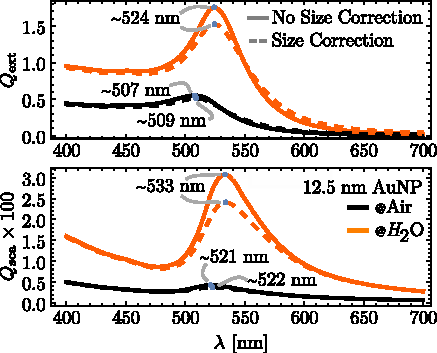
\includegraphics[scale = 1.02]{1-Theory/figs/QextQsca_12-5.pdf}\end{subfigure}
	\hspace*{-.5em}\begin{subfigure}{.05\textwidth}\vspace{-5.5cm}\caption{}\label{sfig:secondaty2}	\end{subfigure}
	\hspace*{-2.em}
	\begin{subfigure}{.48\textwidth} 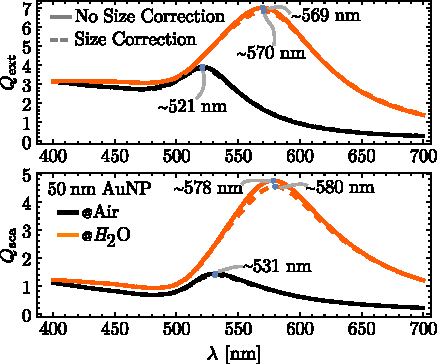
\includegraphics[scale = 1.02]{1-Theory/figs/QextQsca_50.pdf}\end{subfigure}%
\vspace*{-.5em}
\caption[Example of Figure title]{The explanation of your figures. \blindtext}	\label{fig:Main}
\end{figure}

\begin{figure}[h!]\centering
	
\includegraphics[scale=1]{1-Theory/figs/legend.pdf}\\[.5em]
%
	\hspace*{2em}\begin{subfigure}{.05\textwidth}\caption{}\label{sfig:secondary1}\vspace*{6.35cm}\end{subfigure}
	\hspace*{-3.50em}
	\begin{subfigure}{.24\textwidth} 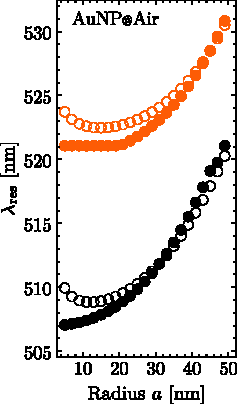
\includegraphics[scale = 1]{1-Theory/figs/redShift_rad1.pdf}\end{subfigure}
%
	\hspace*{.25em}\begin{subfigure}{.05\textwidth}\vspace{-6.35cm}\caption{}\label{sfig:secondaty2}	\end{subfigure}
	\hspace*{-2.5em}
	\begin{subfigure}{.24\textwidth} 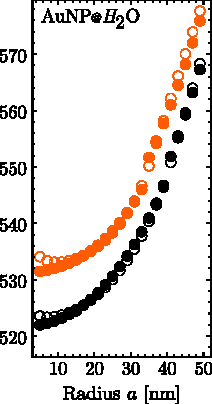
\includegraphics[scale = 1]{1-Theory/figs/redShift_rad2.pdf}\end{subfigure}%
%
	\hspace*{-.5em}\begin{subfigure}{.05\textwidth}\vspace{-6.35cm}\caption{}\label{sfig:secondaty2}	\end{subfigure}
	\hspace*{-2.45em}
	\begin{subfigure}{.24\textwidth} 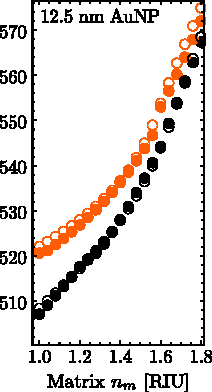
\includegraphics[scale = 1.02]{1-Theory/figs/redShift_mat1.pdf}\end{subfigure}%
%
	\hspace*{-.45em}\begin{subfigure}{.05\textwidth}\vspace{-6.35cm}\caption{}\label{sfig:secondaty2}	\end{subfigure}
	\hspace*{-2.45em}
	\begin{subfigure}{.24\textwidth} 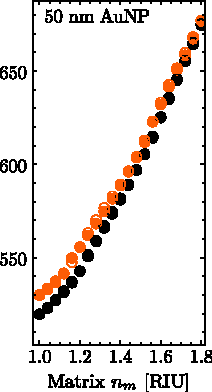
\includegraphics[scale = 1.02]{1-Theory/figs/redShift_mat2.pdf}\end{subfigure}%
\vspace*{-.5em}
\caption[Example of Figure title]{The explanation of your figures. \blindtext}
\label{fig:Main}
\end{figure}
\clearpage


	\section{Mie Scattering}
	  \label{s:Mie}

     In the previous section, it was concluded that the extinction of light due to the interaction between a particle and a monochromatic plane wave can be determinated through the amplitude of the scattered field in the forward direction. This is stated in the Optical Theorem, which is an exact relation, but inaccuracies can arise when either the scattering amplitude matrix or extinction cross section is approximated\footnote{See for example Section 2.4 from Ref. \cite{tsang_scattering_2000} on the Rayleigh Scattering and Section 21.7 from Ref. \cite{zangwill_modern_2013} on Thompson scattering.}. A particular case in which the scattering amplitude matrix can be exactly calculated is when the scatterer has spherical symmetry. In order to address this special case it will be introduced a vectorial basis with spherical symmetry, known as the Vector Spherical Harmonics (VSH)\index{Scattering!Thompson}\index{Scattering!Rayleigh}\index{Spherical!Vector Spherical Harmonics}. Once the SVH are defined, they will be used to write a monochromatic plane wave and, lastly, the scattered field by a spherical particle will be calculated by imposing the continuity of the tangential components of the electric and magnetic field. The optical properties of a gold nanoparticle with a radius of $12.5$ nm are calculated as an example of the developed theoretical framwork in the last section.

	    \subsection{Vector Spherical Harmonics}
		 \label{ss:VSH}
		 % !TeX root = ../tesis.tex

The electric and magnetic field, denoted as $\vb{E}$ and $\vb{B}$, respectively, are a solution to the homogeneous vectorial Helmholtz\index{Helmholtz!Equation, Vectorial} when an harmonic time dependence and a spacial domain with no external charge nor current densities is assumed, that is,
%
% -----------------------------
\begin{subequations}
\begin{tcolorbox}[title = Vectorial Helmholtz Equation,	ams align, breakable]
	\grad^2 \vb{E}(\vb{r},\omega) + k^2 \vb{E}(\vb{r},\omega) &= \vb{0},\\
  \grad^2 \vb{B}(\vb{r},\omega) + k^2 \vb{B}(\vb{r},\omega) &= \vb{0}.
\end{tcolorbox}
\label{eq:Helmholtz}
\end{subequations}
% ------------------------------
%
\noindent where the vectorial operator $\grad^2$ must be understood as $\grad^2 = \nabla(\nabla\cdot) - \nabla\times\nabla\times $, and $k$ is the wave number in the matrix. It is possible to build a basis set for the electric and magnetic fields as long as the elements of this basis are also solution to Eq. \eqref{eq:Helmholtz}. One alternative is to employ the following set of vector functions
%
% -----------------------------
\begin{subequations}
\begin{align}
	\vb{L} =& \nabla \psi,
	\label{eq:L}\\
	\vb{M} =& \nabla\times(\vb{r}\psi),
	\label{eq:M}\\
	\vb{N} =&  \frac{1}{k}\nabla\times\vb{M},
	\label{eq:N}
\end{align}%
\label{eq:VSH}%
\end{subequations}
% ------------------------------
%
that are solution to the homogeneous vectorial Helmholtz equation as long as the scalar function $\psi$ is solution to the scalar Helmholtz equation\footnote{%
	This result can be proven by considering the following: Let $f$ be $\mathcal{C}^3$ and $\vb{F}$ a $\mathcal{C}^2$. Then, it is true that $\nabla^2(\nabla f) = \nabla(\nabla^2 f)$, and $\curl(\grad^2\vb{F}) = \grad^2(\curl\vb{F})$. }\index{Helmholtz!Equation, Scalar}
%
% -----------------------------
\begin{align}
	\nabla^2 \psi + k^2 \psi = 0.
\label{eq:HelmoltzScalar}
\end{align}
% ------------------------------
%
The triad $\left\{\vb{L},\vb{M},\vb{N}\right\}$ is a set of vectors\footnote{%
	Employing the Einstein sum convention with $\epsilon_{ijk}$ the Levi-Civita symbol, Eq. \eqref{eq:M} can be the written as follows:%
	 	$M_i = [\nabla\times(\vb{r}\psi)]_i
	 	=  \epsilon_{ijk}\partial_j(r_k\psi)
	 	=\psi\epsilon_{ijk}\partial_j(r_k) -\epsilon_{ikj}r_k\partial_j\psi
	 	=\psi[\nabla\times\vb{r}]_i - [\vb{r}\times\nabla\psi]_i
	 	= - [\vb{r}\times\nabla\psi]_i
	 	= [\vb{L}\times\vb{r}]_i$,%
	 therefore $\vb{M}$ is orthogonal to $\vb{L}$ and $\vb{r}$. From Eq. \eqref{eq:N} $\vb{M}\cdot\vb{N}=0$, so $\vb{M}$ is orthogonal to $\vb{M}$. As it will be shown, not necessarily $\vb{L}$ is orthogonal to $\vb{N}$.
	}%
that obey Helmholtz equation \textit{i.e.}, they can be directly identify as electric or magnetic fields. The elements of the vector basis from Eq. \eqref{eq:VSH}   are known as the Vectorial Spherical Harmonics (VSH) as defined by  \citeauthor{stratton_electromagnetic_2012} \cite{stratton_electromagnetic_2012}, and \citeauthor{bohren_absorption_1983} \cite{bohren_absorption_1983} and the scalar function $\psi$ is known as the generating function of the VSH. From the definition of the VSH in Eqs. \eqref{eq:VSH} it can be seen that $\vb{L}$ has only a longitudinal component while $\vb{M}$ and $\vb{N}$ have only transversal components; specifically $\vb{M}$ is tangential to any sphere of radius $\norm{\vb{r}}$.


If spherical coordinates are chosen, and it is assumed that $\psi(r,\theta,\varphi) = R(r)\Theta(\theta)\Phi(\varphi)$, then Eq. \eqref{eq:HelmoltzScalar} can be decouple into three ordinary differential equations:
%
% ------------------------------
 \begin{align}
	\frac{1}{\Phi}\pdv[2]{\psi}{\varphi} &+ m^2 \Phi =0,
 \label{eq:Phi}\\
	\frac{1}{\sin\theta}\dv{\theta}\qty(\sin\theta\dv{\Theta}{\theta}) &+ \qty[\ell(\ell+1)- \frac{m^2}{\sin^2\theta}]\Theta =0,
	\label{eq:Theta}\\
	\dv{r}\qty(r^2\dv{R}{r}) &+ \qty[ (k r)^2 - \ell (\ell +1)] R =0,
 \label{eq:Req}
\end{align}	
% ------------------------------
%
where $\ell$ can takes natural values and zero, and $\abs{m}\leq \ell$ so $\Phi$ and $\Theta$ are univalued and finite on a sphere. Eqs. \eqref{eq:Theta} and \eqref{eq:Req} can be rewritten as
%
% ------------------------------
 \begin{align}
(1-\mu^2)\dv[2]{\Theta}{\mu} - 2\mu\dv{\Theta}{\mu} + \qty[\ell(\ell+1)-\frac{m^2}{1-\mu^2}]\Theta &= 0, \qqtext{ with $\mu = \cos\theta$,}
	\label{eq:ThetaMu}\\
	\rho\dv{\rho}\qty(\rho\dv{Z}{\rho}) +  \qty[\rho^2 - \qty(\ell + \frac12)^2]Z  &= 0,  \qqtext{ with $Z = R\sqrt{\rho}$ and $\rho = kr$.}
\label{eq:Reqkr}
\end{align}	
% ------------------------------
%
The solution to Eq. \eqref{eq:ThetaMu} are the associated Legendre functions $ P_\ell^m(\mu)$ and to Eq. \eqref{eq:Reqkr} the solution is given by the Spherical Bessel Functions of the first ($j_\ell$)  and second ($y_\ell$) kind, and the Spherical Hankel functions of first ($h_\ell^{(1)} = j_\ell + iy_\ell$) and second ( $h_\ell^{(2)} = j_\ell - iy_\ell$)  kind. Following the convention from most literature on Mie Scattering \cite{zangwill_modern_2013}, the solution to Eq. \eqref{eq:Phi} will be decompose in an odd ($o$) and an even ($e$) solution, that is, as sine and cosine functions, thus restricting the values of $m$ to non-negative integers. After this procedure, it is determined that the generating function of the VSH is given by
%
% -----------------------------
\begin{subequations}
\begin{tcolorbox}[title = $\psi$: Generating function of the vectorial spherical harmonics,	ams align, breakable]
	\psi_{e\ell m}(r,\theta,\varphi) =& \cos(m\varphi)P_\ell^m(\cos\theta)z_\ell(kr), 
	\label{eq:psiE}\\ 	
	\psi_{o\ell m}(r,\theta,\varphi) =& \sin(m\varphi)P_\ell^m(\cos\theta)z_\ell(kr).
	\label{eq:psiO}
\end{tcolorbox}
\label{eq:psi}
\end{subequations}
% ------------------------------
%
\noindent%
where $z_\ell$ stands for any of the four solutions to the radial equation [Eq. \eqref{eq:Reqkr}]. Substituting Eq. \eqref{eq:psiE} in Eqs. \eqref{eq:L}--\eqref{eq:N} one finds the even SVH
%
% -----------------------------
\begin{subequations}
\begin{tcolorbox}[title = Even vectorial spherical harmonics,	ams align, breakable]
	\vb{L}_{em\ell} =& k \cos(m\varphi)P_\ell^m(\cos\theta)\dv{z_\ell(kr)} {(kr)}\,\vu{e}_r 
					 +  k\cos(m\varphi) \frac{z_\ell(kr)}{kr}\dv{P_\ell^m(\cos\theta)}{\theta} \,\vu{e}_\theta \notag \\
					& - km \sin(m\varphi) \frac{P_\ell^m(\cos\theta)}{\sin\theta}\frac{z_\ell(kr)}{kr} \,\vu{e}_\varphi 
	\label{eq:Leml}\\
	\vb{M}_{em\ell} = &-m\sin(m\varphi)z_\ell(kr) \frac{P_\ell^m(\cos\theta)}{\sin\theta}\,\vu{e}_\theta
					-\cos(m\theta)z_\ell(kr) \dv{P_\ell^m(\cos\theta)}{\theta}(\cos\theta)\,\vu{e}_\varphi,
	\label{eq:Meml} \\
	\vb{N}_{em\ell} = &\cos(m\varphi) \frac{z_\ell(kr)}{kr} \ell(\ell+1)P_\ell^m(\cos\theta)\,\vu{e}_r 
						+ \cos(m\varphi)  \frac{1}{kr} \dv{[kr\, z_\ell(kr)] }{(kr)}
						\dv{P_\ell^m(\cos\theta)}{\theta}(\cos\theta)\,\vu{e}_\theta \notag\\
						&- m \sin(m\varphi) \frac{1}{kr} \dv{[kr\, z_\ell(kr)] }{(kr)}\frac{P_\ell^m(\cos\theta)}{\sin\theta}
		 \,\vu{e}_\varphi, 
	\label{eq:Neml}	
\end{tcolorbox}
\label{eq:SVHEven}
\end{subequations}
% ------------------------------
%
\noindent where the term $\ell( \ell+1)P_\ell^m$ arises since the associated Legendre functions obeys Eq. \eqref{eq:ThetaMu}. Likewise, the odd SVH are given by
%
% -----------------------------
\begin{subequations}
\begin{tcolorbox}[title = Odd vectorial spherical harmonics,	ams align, breakable]
	\vb{L}_{om\ell} =& k \sin(m\varphi)P_\ell^m(\cos\theta)\dv{z_\ell(kr)} {(kr)}\,\vu{e}_r 
					 +  k\sin(m\varphi) \frac{z_\ell(kr)}{kr}\dv{P_\ell^m(\cos\theta)}{\theta} \,\vu{e}_\theta \notag \\
					& +  km\cos(m\varphi) \frac{P_\ell^m(\cos\theta)}{\sin\theta}\frac{z_\ell(kr)}{kr} \,\vu{e}_\varphi 
	\label{eq:Loml}\\
	\vb{M}_{om\ell} = & m\cos(m\varphi)z_\ell(kr) \frac{P_\ell^m(\cos\theta)}{\sin\theta}\,\vu{e}_\theta
					-\sin(m\theta)z_\ell(kr) \dv{P_\ell^m(\cos\theta)}{\theta}(\cos\theta)\,\vu{e}_\varphi,	
	\label{seq:Moml} \\
	\vb{N}_{om\ell} =&\sin(m\varphi)\frac{z_\ell(kr)}{kr} \ell(\ell+1)P_\ell^m(\cos\theta)\,\vu{e}_r +
					 \sin(m\varphi)  \frac{1}{kr} \dv{[kr\, z_\ell(kr)]}{(kr)} \dv{P_\ell^m(\cos\theta)}{\theta}(\cos\theta) \,\vu{e}_\theta \notag\\
					 & + m \cos(m\varphi) \frac{1}{kr} \dv{[kr\, z_\ell(kr)]}{(kr)} \frac{P_\ell^m(\cos\theta)}{\sin\theta}¸\, \vu{e}_\varphi.
	 \label{seq:Noml} 
\end{tcolorbox}
\label{eq:SVHOdd}
\end{subequations}
% ------------------------------
%
\noindent%
The election on $z_\ell$ in Eqs. \eqref{eq:SVHEven} and  \eqref{eq:SVHOdd} is due to the physical constrains of the scattering problem. The spherical Bessel function of first kind, unlike the other three proposed solution to the radial equation, is finite in $r = 0$, thus it is appropriate for the internal electric field and plane waves. This election of $z_\ell$ will be denoted in the SVH with the superscript $(1)$. On the other hand, the asymptotic behavior of the Hankel function of first kind $h^{(1)} = j_\ell + i y_\ell$ is an outward spherical wave \cite{bohren_absorption_1983}, suited for the scattered field; the VSH with $z_\ell = h^{(1)}\ell$ will be then, denoted with the superscript $(3)$.

The SVH follow orthogonality relations inherited from the orthogonality of sine, cosine and the associated Legendre functions. Let us define the inner product as the integral in the solid angle between two vectorial functions as 
%
\begin{align}
\ev{\vb{A},\vb{A}'}_\Omega = \int_0^{2\pi}\int_0^{\pi} \vb{A}\cdot\vb{A}'\sin\theta\dd{\theta}\dd{\varphi}.
\label{eq:inner}
\end{align}
%
Under this inner product, all even SVH are orthogonal to the odd SVH due to the ortogonallity from the $\sin(m\varphi)$ and $\cos(m'\varphi)$, as well as all SVH  with $m\neq m'$. The remaining orthogonality relations are summarized in the following expressions \cite{stratton_electromagnetic_2012}
%
\begin{align}
\ev{\vb{L}_{em\ell},\vb{L}_{em\ell'}}_\Omega = \ev{\vb{L}_{om\ell},\vb{L}_{om\ell'}}_\Omega &= \delta_{\ell,\ell'}\frac{(1+\delta_{m,0})2\pi}{2\ell+1}\frac{(\ell+m)!}{(\ell-m)!}k^2\qty[ \ell z_{\ell-1}^2(kr) + (\ell+1)z_{\ell+1}^2(kr) ],\\
%
\ev{\vb{M}_{em\ell},\vb{M}_{em\ell'}}_\Omega = \ev{\vb{M}_{om\ell},\vb{M}_{om\ell'}}_\Omega &= \delta_{\ell,\ell'}\frac{(1+\delta_{m,0})2\pi}{2\ell+1}\frac{(\ell+m)!}{(\ell-m)!}\ell(\ell+1)z_{\ell}^2(kr),\\
%
\ev{\vb{N}_{em\ell},\vb{N}_{em\ell'}}_\Omega = \ev{\vb{N}_{om\ell},\vb{N}_{om\ell'}}_\Omega &= \delta_{\ell,\ell'}\frac{(1+\delta_{m,0})2\pi}{(2\ell+1)^2}\frac{(\ell+m)!}{(\ell-m)!}\ell(\ell+1)\qty[ (\ell+1) z_{\ell-1}^2(kr) + \ell z_{\ell+1}^2(kr) ]. \\
%%
\ev{\vb{L}_{em\ell},\vb{N}_{em\ell'}}_\Omega = \ev{\vb{L}_{om\ell},\vb{N}_{om\ell'}}_\Omega &= \delta_{\ell,\ell'}\frac{(1+\delta_{m,0})2\pi}{(2\ell+1)^2}\frac{(\ell+m)!}{(\ell-m)!}\ell(\ell+1)k\qty[ z_{\ell-1}^2(kr) - z_{\ell+1}^2(kr) ]. 
\end{align}
%


















































        \subsection{Incident, Scattered and Internal Electric Fields}
	     \label{ss:Fields}
         % !TeX root = ../tesis.tex

 Let $\vb{E}^{\text{i}}$ be a $x$ polarized plane wave traveling in the vertical direction $\vb{e}_z$; its representation in the canonical spherical basis is
 %
 \begin{align}
 \vb{E}^{\text{i}} (\vb{r})= E_0\qty(\sin\theta\cos\varphi \vu{e}_r +
					\cos\theta\cos\varphi \vu{e}_\theta
					- \sin\varphi \vu{e}_\varphi) \exp(ikr\cos\theta).
	\label{eq:ExPlane}
 \end{align}
 %
The monochromatic plane wave is a transversal wave, thus it can be written in terms of only the VSH $\vb{M}^{(1)}$ and $\vb{N}^{(1)}$, where the radial dependency is given by $j_\ell$ since the monochromatic plane wave is finite everywhere. Even more, due to the dependency on $\varphi$, it is only restricted to values of $m = 1$. By inspection on the radial component of $\vb{E}^\text{i}$, proportional to $\cos\varphi$ it depends only on $\vb{N}_{e1\ell}^{(1)}$, and on the azimuthal component, proportional to $\sin\varphi$, it can depend only on $\vb{M}_{o1\ell}^{(1)}$. Thus, Eq. \eqref{eq:ExPlane} can be written as the linear combination of  $\vb{N}_{e1\ell}^{(1)}$ and $\vb{M}_{o1\ell}^{(1)}$. Through the orthogonality relations of the VSH, the $x$ polarized plane wave can be written as \cite{stratton_electromagnetic_2012}
  %
  \begin{subequations}
 \begin{align}
 \vb{E}^\text{i} (\vb{r})=& E_0 \sum_\ell\frac{i^\ell(2\ell+1)}{\ell(\ell+1)}\qty( \vb{M}_{o1\ell}^{(1)} -i \vb{N}_{e1\ell}^{(1)}),
\\
 \vb{H}^\text{i} (\vb{r})=& \frac{-kE_0}{\mu\omega} \sum_\ell\frac{i^\ell(2\ell+1)}{\ell(\ell+1)}\qty( \vb{M}_{e1\ell}^{(1)} +i \vb{N}_{o1\ell}^{(1)}).
 \end{align}%
 \label{eq:plane waveMultipole}%
   \end{subequations}%
%

In the problem of scattering due to a spherical particle of radius $a$, the continuity conditions on the parallel components on the electric and magnetic fields are written as
  %
 \begin{align}
 \qty(\vb{E}^\text{i} + \vb{E}^\text{sca}- \vb{E}^\text{int})\eval_{r=a}\times \vu{e}_r  =
  \qty(\vb{H}^\text{i} + \vb{H}^\text{sca} - \vb{H}^\text{int})\eval_{r=a} \times\vu{e}_r = 0,
  \label{eq:contuinity}
 \end{align}
 %
with  $\vb{E}^\text{sca}$ ( $\vb{E}^\text{int}$) the scattered (internal) electric field and  $\vb{H}^\text{sca}$ ( $\vb{H}^\text{int}$) the scattered (internal) magnetic field. If the incident field $\vb{E}^\text{i}$ is given by a $x$ polarized plane wave [Eq. \eqref{eq:ExPlane}] then the scattered and internal fields can be written also as a linear combination of $\vb{M}_{o1\ell}$ and $\vb{N}_{e1\ell}$. The internal field is finite inside the particle, thus the radial dependency is given by the function $j_\ell(k_p a)$ with $k_p$ the wave number inside the particle, while it is chosen the spherical Hankel function of first kind $h^{(1)}(ka)$  for the scattered fields due to its asymptotic behavior of a spherical outgoing wave, such election for the radial dependency is denoted by the superscript $(3)$ over the VSH. To simplify the following steps, the scattered and the internal electric files are proposed as
  %
  \begin{subequations}
 \begin{align}
 \vb{E}^\text{sca} (\vb{r})=& E_0 \sum_\ell\frac{i^\ell(2\ell+1)}{\ell(\ell+1)}\qty(i a_\ell \vb{N}_{e1\ell}^{(3)} -b_\ell \vb{M}_{o1\ell}^{(3)}),
 \label{eq:EscaLC}\\
 \vb{E}^\text{int} (\vb{r})=& E_0 \sum_\ell\frac{i^\ell(2\ell+1)}{\ell(\ell+1)}\qty( c_\ell\vb{M}_{o1\ell}^{(1)} - i d_\ell \vb{N}_{e1\ell}^{(1)}),
 \end{align}
 \label{eq:EscaInt}
 \end{subequations}
 %
% where the Hankel spherical functions has $\rho =$
with the respective magnetic fields
  %
    \begin{subequations}
 \begin{align}
 \vb{H}^\text{sca} (\vb{r})=& \frac{-kE_0}{\mu\omega} \sum_\ell\frac{i^\ell(2\ell+1)}{\ell(\ell+1)}\qty(i b_\ell \vb{N}_{o1\ell}^{(3)} +a_\ell \vb{M}_{e1\ell}^{(3)}),\\
 \vb{H}^\text{int} (\vb{r})=& \frac{-kE_0}{\mu_p\omega} \sum_\ell\frac{i^\ell(2\ell+1)}{\ell(\ell+1)}\qty( d_\ell\vb{M}_{e1\ell}^{(1)} + i c_\ell \vb{N}_{o1\ell}^{(1)}).
 \end{align}%
\label{eq:HscaInt}%
 \end{subequations}%
 %
Since only the term $m=1$ is taken into account, it is convenient to define the angular functions
%
\begin{align}
 \pi_\ell(\cos\theta )  = \frac{P_\ell^1(\cos\theta)}{\sin\theta},\qqtext{and}
 \tau_\ell(\cos\theta) = \dv{P_\ell^1(\cos\theta)}{\theta},
 \label{eq:PiTau}
\end{align}
%
which are not orthogonal but their addition and substraction are, that is $\pi_\ell \pm \tau_\ell$ are orthogonal functions \cite{bohren_absorption_1983}. After substitution  of Eqs. \eqref{eq:plane waveMultipole}, \eqref{eq:EscaInt} and \eqref{eq:HscaInt} into Eq. \eqref{eq:contuinity} and considering the orthogonality of the odd and even VSH, of the vectors $\vb{M}$ and $\vb{N}$, and of $\pi_\ell \pm \tau_\ell$, it is shown that the coefficients $a_\ell$, $b_\ell$, $c_\ell$ and $d_\ell$ are given by two decoupled equation systems
%
\begin{align}
\mqty([x h_\ell^{(1)}(x)]  & (\mu/\mu_p) [(mx) j_\ell(mx)] \\
		m[x h_\ell^{(1)}(x)]' & [(mx) j_\ell(mx)]')
		\mqty(a_\ell \\ d_\ell) = \mqty([xj_\ell(x)] \\ m[x j_\ell(x)]') ,
	\label{eq:syst1}
		\\
\intertext{and}
\mqty( m[xh_\ell^{(1)}(x)]  &  [(mx)j_\ell(mx)] \\
		[x h_\ell^{(1)}(x)]' & (\mu/\mu_p)[(mx) j_\ell(mx)]' )
		\mqty(b_\ell \\ c_\ell) = \mqty(m[xj_\ell(x)] \\ [x j_\ell(x)]'),
	\label{eq:syst2}
\end{align}
%
where $m = k_p / k = n_p / n_\text{m}$ is the contrast between the sphere and the matrix, $x= ka = 2\pi n_\text{m} (a/\lambda)$ is the size parameter and  ($'$) denotes the derivative respect to the argument of the spherical Bessel or Hankel functions. The Eqs. \eqref{eq:syst1} and \eqref{eq:syst2} are simplified when the Riccati-Bessel functions $\psi_\ell( \rho) = \rho j_\ell(\rho)$ and $\xi(\rho) = \rho h_\ell^{(1)}(\rho)$ are introduced.

When a no magnetic particle nor matrix are assumed  ($\mu_p = \mu = \mu_0$), the coefficients $a_\ell$ and $b_\ell$ are known as the Mie Coefficients whose expression is calculated by inverting  Eqs. \eqref{eq:syst1} and \eqref{eq:syst2}, leading to
% -----------------------------
\begin{subequations}
	\begin{tcolorbox}[title = Mie Coefficients, ams align, breakable ]
	a_\ell &= \frac{\psi_\ell(x)\psi_\ell' (mx)-m\psi_\ell(mx)\psi_\ell'(x)}
				{\xi_\ell(x)\psi_\ell'(mx)-m\psi_\ell(mx)\xi_\ell'(x)},
				\label{eqs:a_ell}\\[.5em]
	b_\ell &= \frac{m\psi_\ell(x)\psi_\ell' (mx)-\psi_\ell(mx)\psi_\ell'(x)}
			{m\xi_\ell(x)\psi_\ell'(mx)-\psi_\ell(mx)\xi_\ell'(x)}.
			 \label{eqs:b_ell}
	\end{tcolorbox}\label{eq:MieCoef}
\end{subequations}
% ------------------------------
\noindent
Likewise, the coefficients $c_\ell$ and $d_\ell$ are
% -----------------------------
\begin{subequations}
\begin{align}
	c_\ell &= \frac{-m\xi_\ell'(x)\psi_\ell(x)+m\xi_\ell(x)\psi_\ell'(x)}
			{m\xi_\ell(x)\psi_\ell'(mx)-\psi_\ell(mx)\xi_\ell'(x)},\\[.5em]
	d_\ell &= \frac{-m\xi'_\ell(x)\psi_\ell(x)+m\psi_\ell'(mx)\psi_\ell'(x)}
				{\xi_\ell(x)\psi_\ell'(mx)-m\psi_\ell(mx)\xi_\ell'(x)}.
\end{align}%
\label{eq:coeffInt}%
\end{subequations}\noindent%
% ------------------------------
%
Even though the coefficients of the linear combination for the scattered and internal fields were obtained by assuming an $x$ polarized incident field, due to the spherical symmetry of the problem, by applying the transformation $\varphi \to \varphi + \pi/2$  the same procedure is valid for a $y$ polarized incident field  \cite{bohren_absorption_1983}, therefore all quantities related to the scattered and the internal field can be expressed in terms of Eqs. \eqref{eq:MieCoef} and \eqref{eq:coeffInt}.

As discussed in Section \ref{section:AmpMatCrossSect}, the optical properties of a particle are codified into the scattering, absorption and extinction cross sections, quantities that can be calculated by means of the scattering amplitude matrix [Eq. \eqref{eq:ScatAmpMat}] and the Optical Theorem [Eq. \eqref{eq:Cext}]. Since the particle is spherical, it is convinient to exploit the symmetry of the problem  by decomposing the scattered electric field [Eq. \eqref{eq:EscaLC}] into components parallel and perpendicular to the scattering plane. To obtain the scattering amplitude matrix  expressed in an orthogonal base relative to the scattering plane ($\vu{e}_\parallel^s =\vu{e}_\theta$ and $\vu{e}_\perp^s=-\vu{e}_\varphi$) let us substitute the Mie Coefficients [Eq. \eqref{eq:MieCoef}] into Eq. \eqref{eq:EscaLC}  while rewriting the VSH $\vb{M}^{(3)}_{o1\ell}$  [Eq. \eqref{eq:Moml}] and $\vb{N}^{(3)}_{e1\ell}$ [Eq. \eqref{eq:Neml}] in terms of the Riccati-Bessel function  $\xi$ and its derivative:
%
\begin{subequations}\label{eq:Esca}%
\begin{align}
\vb{E}^\text{sca}\cdot\vu{e}_r &=  \frac{\cos\varphi}{(kr)^2}
								\sum_\ell^\infty E_0i^\ell(2\ell+1)
								ia_\ell \xi(kr)\pi_\ell(\cos\theta) \sin\theta ,
\label{eq:EscaR}\\
\vb{E}^\text{sca}\cdot\vu{e}^\text{sca}_\parallel &=  \frac{\cos\varphi}{kr}
								\sum_\ell^\infty E_0i^\ell\frac{2\ell+1}{\ell(\ell+1)}
						[i a_\ell\xi_\ell'(kr)\tau_\ell(\cos\theta)-b_\ell\xi_\ell(kr)\pi_\ell(\cos\theta)],
\label{eq:EscaTheta}\\
\vb{E}^\text{sca}\cdot\vu{e}^\text{sca}_\perp &=  \frac{\sin\varphi}{-kr}
								\sum_\ell^\infty E_0i^\ell\frac{2\ell+1}{\ell(\ell+1)}
						[i a_\ell\xi_\ell'(kr)\pi_\ell(\cos\theta)-b_\ell\xi_\ell(kr)\tau_\ell(\cos\theta)].
\label{eq:EscaMPhi}
\end{align}%
\end{subequations}
%
Following a similar procedure but substituting Eq. \eqref{eq:coeffInt} into Eq. \eqref{eq:EscaInt}, the internal electric field $\vb{E}^\text{int}$ can be rewritten also in terms of the Riccati-Bessel functions as

\begin{subequations}\label{eq:Eint}%
\begin{align}
\vb{E}^\text{int}\cdot\vu{e}_r &=  -\frac{\cos\varphi}{(kr)^2}
               \sum_\ell^\infty E_0i^\ell(2\ell+1)
               id_\ell \psi(kr)\pi_\ell(\cos\theta) \sin\theta ,
\label{eq:EintR}\\
\vb{E}^\text{int}\cdot\vu{e}^\text{sca}_\parallel &=  \frac{\cos\varphi}{kr}
               \sum_\ell^\infty E_0i^\ell\frac{2\ell+1}{\ell(\ell+1)}
           [-i d_\ell\psi_\ell'(kr)\tau_\ell(\cos\theta)+c_\ell\psi_\ell(kr)\pi_\ell(\cos\theta)],
\label{eq:EscaTheta}\\
\vb{E}^\text{int}\cdot\vu{e}^\text{sca}_\perp &=  \frac{\sin\varphi}{-kr}
               \sum_\ell^\infty E_0i^\ell\frac{2\ell+1}{\ell(\ell+1)}
           [-i d_\ell\psi_\ell'(kr)\pi_\ell(\cos\theta)+c_\ell\psi_\ell(kr)\tau_\ell(\cos\theta)].
\label{eq:EintMPhi}
\end{align}%
\end{subequations}


The scattering amplitude matrix relates the incident electric field to the scattered electric field in the far field regime, that its when $kr\gg 1$. Considering that the series of Eqs. \eqref{eq:EscaR}-\eqref{eq:EscaMPhi} converge uniformly, so all contributions after the sufficiently large  term $\ell_c$ of the sum can be neglected for all values of $kr$, the asymptotic  expressions for the $\xi$ Riccati-Bessel function and its derivative can be employed, which are \cite{bohren_absorption_1983}
%
\begin{align}
\xi(kr)\approx (-i)^\ell \frac{\exp(ikr)}{i},
\qqtext{and}
\dv{\xi(kr)}{(kr)} = (-i)^\ell \exp(ikr)\qty(\frac{1}{i kr} + 1),
\qqtext{when}
\ell_c^2\ll kr.
\label{eq:RBXiAssym}
\end{align}
%

Substituting Eq. \eqref{eq:RBXiAssym} into  Eqs. \eqref{eq:EscaR}-\eqref{eq:EscaMPhi} and depreciating all terms proportional to $(kr)^{-2}$ it leads to a zero radial electric field while
%
\begin{subequations}%
\begin{align}
\vb{E}^\text{sca}\cdot\vu{e}^\text{sca}_\parallel & \approx \frac{\exp(ikr)}{r}
\left\{\frac{i}{k}\sum_\ell^\infty \frac{2\ell+1}{\ell(\ell+1)}
						[a_\ell\tau_\ell(\cos\theta)+b_\ell\pi_\ell(\cos\theta)]
				\right\}E_0\cos\varphi,
\label{eq:EthetaSca}\\
\vb{E}^\text{sca}\cdot\vu{e}^\text{sca}_\perp &\approx \frac{\exp(ikr)}{r}
\left\{\frac{i}{k}\sum_\ell^\infty \frac{2\ell+1}{\ell(\ell+1)}
						[a_\ell\pi_\ell(\cos\theta)+b_\ell\tau_\ell(\cos\theta)]
				\right\}E_0(-\sin\varphi),
\label{eq:EphiSca}
\end{align}\label{eq:EFar}
\end{subequations}
%
where it can be identified that $\vb{E}^\text{i}\cdot \vu{e}^\text{i}_\parallel = E_0\cos\varphi$ and $\vb{E}^\text{i}\cdot \vu{e}^\text{i}_\perp = -E_0\sin\varphi$ for $\vb{E}^\text{i}$ a plane wave traveling along the $z$ direction with an arbitrary polarization. Finally, the Scattering Amplitude Matrix for a spherical particle can be obtained by comparing Eqs. \eqref{eq:EthetaSca} and \eqref{eq:EphiSca} with Eq. \eqref{eq:ScatAmpMat}, leading to
%
\begin{tcolorbox}[title = Scattering Amplitude Matrix for Spherical Particles, ams align, breakable ]
\mathbb{F}(\vu{k}^\text{sca},\vu{k}^\text{i})
            &= \mqty(\dfrac{i}{k}S_2(\theta) & 0 \\
			0 & \dfrac{i}{k}S_1(\theta)  ),
            \label{eq:FscaS}
\intertext{with  $\vu{k}^\text{sca} = \vu{e}_r$, $\vu{k}^\text{i} = \vu{e}_z$, $\cos\theta = \vu{k}^\text{sca}\cdot\vu{k}^\text{i}$  and}
S_1(\theta)  &= \sum_\ell^\infty \frac{2\ell+1}{\ell(\ell+1)}
						[a_\ell\tau_\ell(\cos\theta)+b_\ell\pi_\ell(\cos\theta)],
            \label{eq:S1}
\\
S_2(\theta) &= \sum_\ell^\infty \frac{2\ell+1}{\ell(\ell+1)}
						[a_\ell\pi_\ell(\cos\theta)+b_\ell\tau_\ell(\cos\theta)].
            \label{eq:S2}
\end{tcolorbox}
%
The scattering amplitude matrix $\mathbb{F}$ shows the symmetry of the system when written in the a base relative to the scattering plane direction, as it was stated in Sec. \ref{section:AmpMatCrossSect}. Since the scatterer is a spherical istropic NP,  $\mathbb{F}$ is a diagonal matrix in the base  $\{\vu{e}^\text{sca}_\parallel, \vu{e}^\text{sca}_\perp  \}$, that is, that the scattered electric field $\vb{E}^\text{sca}$ mantains the same polarization degree relative to the scattering plane than the incident electric field $\vb{E}^\text{i}$ that illuminates the spherical particle.


        \subsection{Near and Far Field Regimes: Optical Properties of Single Spherical Particles}
		 \label{ss:AuMie}

         In the previous sections, the general theory for the light scattering was developed, introducing the amplitude scattering matrix $\mathbb{F}$ [Eq. \eqref{eq:ScatAmpMat}]. Then, the particular problem of a spherical symmetric scatterer was addressed and the explicit expression of the scattered electric field and of $\mathbb{F}$ were obtained [Eq. \eqref{eq:FscaS}] in terms of the Mie coefficients $a_\ell$ and  $b_\ell$ [Eqs. \eqref{eq:MieCoef}], as well as the internal electric field inside the scatterer [Eq. \eqref{eq:EFar}] in terms of the coefficients $c_\ell$ and $d_\ell$ [Eqs. \eqref{eq:coeffInt}]. The  optical properties of a particle is related to the the electric field outside the scatterer,  and can be studied within two different spacial regions: the near field and the far field regimes. The near field regime consists in the complete analytical solution of the scattered electric field [Eq. \eqref{eq:EscaLC}], while the far field regime considers only its contributions proportional to $r^{-1}$, with $r$ the distance between the center of the scatterer and the measurement point, which can be determined by the amplitude scattering matrix $\mathbb{F}$ alone.  In this last section,
                the past results are employed to calculate the optical properties for a spherical gold nanoparticle (AuNP) with a radius of $12.5$ nm embedded into a matrix of air and into a matrix of glass when it is illuminated by an incident plane wave with a wavelength $\lambda$.

            \subsubsection{Localized Surface Plasmon}
             \label{sss:LSPR}
             % !TeX root = ../tesis.tex

The optical properties of a particle, either in the near or the far field regime,  are determined by the Mie coefficients   $a_\ell$ and $b_\ell$ [Eq. \eqref{eq:MieCoef}] since the exact solution to the scattered electric field $\vb{E}^\text{sca}$ is a linear combination of the vector spherical harmonics (VSH) $\vb{N}^{(3)}_{\text{e}1\ell}$ and $\vb{M}^{(3)}_{\text{o}1\ell}$ [Eq. \eqref{eq:EscaLC}] modulated by  $a_\ell$ and $b_\ell$, respectively. Thus, the physical interpretation of each term $\ell$ in the linear combination, as well as of $\vb{N}^{(3)}_{\text{e}1\ell}$ and $\vb{M}^{(3)}_{\text{o}1\ell}$ can be determined by visualizing each one of them independently. By understanding the contribution of each term, the optical response of a particle illuminated by a plane wave can be studied in the near and far regime.

The Fig. \ref{fig:Multipoles} shows the decomposition of the the scatttered electric field  $\vb{E}^\text{sca}$ of a particle into its contributions proportional to $a_1$ [Fig. \ref{fig:VSH:a1}], $b_1$ [Fig. \ref{fig:VSH:b1}], $a_2$ [Fig. \ref{fig:VSH:a2}] and $b_2$ [Fig. \ref{fig:VSH:b2}], when the particle is illuminated by a $x$ polarized plane wave traveling in the $z$ direction. The vectorial behavior of the $a_\ell$ contributions to $\vb{E}^\text{sca}$ are given by the VSH $\vb{N}^{(3)}_{\text{e}\ell 1}$ and by $\vb{M}^{(3)}_{\text{o}\ell 1}$ for the $b_\ell$ contributions. The  scattered electric field  is evaluated at a spherical surface (gray sphere) larger than the scatter: the arrow stream on the spherical surface corresponds to the pointing direction of each contribution to $\vb{E}^\text{sca}$ parallel to the evaluation sphere, while the color code corresponds to the magnitude of the scattered electric field at each point; the solid shape at the center of each axis is a contour surface $\norm{\vb{E}^\text{sca}}$.
%

\begin{figure}[h!]
	\def\svgwidth{1\textwidth} \small
  \vspace*{3.0em}
  \hspace*{0.em}
    \begin{subfigure}{.24\textwidth}\caption{\centering $\vb{E}^\text{sca} \sim  i a_1 \vb{N}^{(3)}_{\text{e}11}$}\label{fig:VSH:a1}\end{subfigure}
  	\begin{subfigure}{.24\textwidth}\caption{\centering $\vb{E}^\text{sca} \sim  - b_1 \vb{M}^{(3)}_{\text{o}11}$}\label{fig:VSH:b1}\end{subfigure}
	\begin{subfigure}{.24\textwidth}\caption{\centering $\vb{E}^\text{sca} \sim  i a_2 \vb{N}^{(3)}_{\text{e}12}$}\label{fig:VSH:a2}\end{subfigure}
	\begin{subfigure}{.24\textwidth}\caption{\centering $\vb{E}^\text{sca} \sim  - b_2 \vb{M}^{(3)}_{\text{o}12}$}\label{fig:VSH:b2}\end{subfigure}
  \vspace*{-6.em}\\
  \includeinkscape{VSH/3-VSH}
  \vspace*{-2em}
  \caption[Multipolar Contributions to the Scattered Electric Field]{ Decomposition of the  scattered electric field $\vb{E}^\text{sca}$ into its contributions  proportional to \textbf{a)} $a_1$,  \textbf{b)}  $b_1$, \textbf{c)} $a_2$ and \textbf{d)} $b_2$ [see Eq. \eqref{eq:EscaLC}] when a particle (not shown) is illuminated by an $x$ polarized plane wave traveling in the $z$ direction. The scattered electric field $\vb{E}^\text{sca}$ is evaluated at a sphere larger than the particle: the arrow stream corresponds to the projection parallel to the evaluation sphere of $\vb{E}^\text{sca}$  and the color code corresponds to the magnitude of  $\vb{E}^\text{sca}$. A contour surface of the magnitude of $\vb{E}^\text{sca}$ is located at the center of each axis. }
\label{fig:Multipoles}
\end{figure}

The general effect of each contribution to the scattered electric field  $\vb{E}^\text{sca}$  can be understood by analyzing their the behavior around the points where the scattered electric field drops to  zero; such points are called nodes and are shown in dark bluish colors in  Fig. \ref{fig:Multipoles}. The number of nodes over the evaluation sphere (gray surface) is proportional to the chosen value of $\ell$, for example, if $\ell = 1$ [Figs. \ref{fig:VSH:a1} and \ref{fig:VSH:b1}] there is a pair of such nodes and if $\ell = 2$ [Figs. \ref{fig:VSH:a2} and \ref{fig:VSH:b2}] there are two pairs, where each pair consists of two nodes at opposite sides of the evaluation sphere. When comparing the contributions proportional to $a_\ell$ [Figs. \ref{fig:VSH:a1} and \ref{fig:VSH:a2}] and  to $b_\ell$ [Figs. \ref{fig:VSH:b1} and \ref{fig:VSH:b2}], one difference is the location of the pairs of nodes for a fixed value of $\ell$, which differ spatially by a rotation around the $z$ axis of an angle $\varphi = \pi/2$.  Another difference between the $a_\ell$ and the $b_\ell$ contribution to  $\vb{E}^\text{sca}$ are the trajectories they performed around each pair of nodes: the $a_\ell$ contributions the scattered electric field flows from one node to its pair, thus following an open path, while the scattered electric field for the $b_\ell$ contributions circulates around the nodes forming a closed path. Taking into account such behaviors of the scattered electric field, it can be seen that the $a_\ell$ ($b_\ell$) contribution describes the electric field of an electric (magnetic) dipole when $\ell = 1$ and of an electric (magnetic) quadrupole when $\ell = 2$. Extrapolating such behavior for an arbitrary $\ell$,  it can be concluded that the $a_\ell$ contributions to the scattered electric field, described by the VSH $\vb{N}^{(3)}_{\text{e}\ell 1}$ corresponds to the electric field of an electric multipole of order $\ell$, while the $b_\ell$ contribution, described by the VSH $\vb{M}^{(3)}_{\text{o}\ell 1}$, corresponds to the electric field of a magnetic multipole of order $\ell$.

The scattered electric field of a spherical particle can be written, according to Eq. \eqref{eq:EscaLC}, as a linear contribution of electric fields associated to electric and magnetic mulutipoles as shown in Fig. \ref{fig:Multipoles}, modulated by the Mie coefficients $a_\ell$ and $b_\ell$, respectively. The Mie coefficients [Eq. \eqref{eq:MieCoef}] have a dependency on the radius $a$ of the spherical particle, on the wavelength $\lambda$ of the incident plane wave, the matrix embedding the particle through its  refractive index $n_\text{mat} = \sqrt{\varepsilon_\text{m}/\varepsilon_0}$, with $\varepsilon_\text{m}$ its dielectric function, and on the material of the particle itself, also through its refractive index $n_\text{p} = \sqrt{\varepsilon_\text{p}/\varepsilon_0}$, where $\varepsilon_p$ is the dielectric function of the particle, which in general depends on the wavelength of the incident plane wave.


            \subsubsection{Far Field Optical Propterties}
             \label{sss:FarField}
             % !TeX root = ../tesis.tex


In Fig. \ref{fig:Mieefficiencies} the extinction  $Q_\text{ext}$ and the scattering  $Q_\text{sca}$ efficiencies of a gold NP (AuNP) with a radius of $a = 12.5$ nm (12.5 nm AuNP) are shown as function of the wavelength $\lambda$ of the incident plane wave illuminating the NP. Two matrices were considered in Fig. \ref{fig:Mieefficiencies}: a matrix of air with a refractive index of $n_\text{mat} = 1$ (black lines) and a matrix of glass with $n_\text{mat} = 1.5$ (orange lines).  The experimental dielectric function for Au reported by \citeauthor{johnson_optical_1972} \cite{johnson_optical_1972}  was employed to model the electromagnetic response of the spherical AuNP nevertheless, this data corresponds to a bulk sample, meaning that it may not reproduce the optical behavior of a NP since surface effects cease to be neglectable  due to their spacial dimensions \cite{noguez_surface_2007}.   In order to study  the optical properties of AuNP while considering  surface effects,  a size correction to the dielectric function of the AuNP was performed as described in Appendix \ref{app:SizeCorrection}. The efficiencies of the $12.5$ nm AuNP  taking into account a dielectric function with (dashed lines) and without (solid lines) a size correction were compared for both considered matrices; on each curve the wavelength of their maximum value is indicated. The value of $\lambda$ at which the extinction efficiency is maximum corresponds to the excitation wavelength of the Localized Surface Pasmon Resonance (LSPR), that is, the wavelength where the extinction of light occurs the most.

% -------------------------------------- Extinctintion and scattering efficiencies -------------------------------
% --------------------------------------          12.5 nm AuNP @ Air and @ glass   -------------------------------
% --------------------------------------               fig:Mieefficiencies         -------------------------------
\begin{figure}[h!]
	\def\svgwidth{1\textwidth} \small
  \vspace*{3.0em}
  \hspace*{-9.em}
    \begin{subfigure}{.46\textwidth}\caption{ }\label{fig:Mieefficiencies:a}\end{subfigure}
    \begin{subfigure}{.49\textwidth}\caption{ }\label{fig:Mieefficiencies:b}\end{subfigure}
  \vspace*{-6.em}\\
  \includeinkscape{Mie-Au/1-Efficiencies}
  \vspace*{-2em}
  \caption[Extinction and Scattering Efficency of a 12.5 nm Au Spherical NP embeded into Air and Glass]{ \textbf{a)} Extinction $Q_\text{ext}$ and \textbf{b)} scattering $Q_\text{sca}$ efficiencies of a 12.5 nm Au spherical NP embeded into air (black, $n_\text{mat} = 1$)  and into galss (orange, $n_\text{mat} = 1.33$), as function of the wavelength $\lambda$ of the incident plane wave.  The solid curves were calculated by considering no size effects on the dielectric function of the AuNP, while the dashed curves consider a size correction to it; the experimental data of \citeauthor{johnson_optical_1972} \cite{johnson_optical_1972} was employed.}
\label{fig:Mieefficiencies}
\end{figure}
% --------------------------------------               fig:Mieefficiencies         -------------------------------

From the extinction and scattering efficiencies in Fig. \ref{fig:Mieefficiencies}, two main spectral tendencies arises between these quantities: on the overall value of the efficiencies and on the spectral position of their maximum. Since the scattering efficiency is two orders of magnitude smaller than the extinction efficiency within the visible range, the main energy loss mechanism is absorption, as stated by the Optical Theorem [Eq. \eqref{eq:Cext}]. Even though the 12.5 nm AuNP absorbs more light than what it scatters, both phenomena are present. For example, when the  12.5 nm AuNP is embedded into air, the wavelengths at which it absorbs and scatters the most are $\sim 509$ nm and $\sim 522$ nm, respectively. When the AuNP is embedded into glass, the absorption of light is optimized at a wavelength of $\sim 535$ nm, while the scattering is optimized at $\sim 543$ nm. For both an air and a glass matrix, the wavelength of most scattering is redshifted relative to the wavelength of most absorption for each case: $\sim 15$ nm for air and $\sim 7$ nm for glass. The extinction and scattering have different spectral tendencies as already discussed, yet they share common characteristics   when the dependency on the embedding media is studied.

Both the scattering and the absorption efficiencies of a 12.5 nm AuNP present an overall enhancement within the visible range when the refractive index of the matrix, the embedding media,  increases. This can be seen in Fig. \ref{fig:Mieefficiencies} by comparing the black curves ($n_\text{mat} = 1$, air) with the orange curves ($n_\text{mat} = 1.5$, glass). The value of the extinction efficiency of a 12.5 nm AuNP  at the excitation wavelength of the LSPR for a matrix of glass is around five times larger than for a matrix of air, as it can bee seen in Fig. \ref{fig:Mieefficiencies:a}, while the maximum value of the scattering efficiency for a glass matrix is around eight times larger compared to the case of an air matrix, as shown in Fig. \ref{fig:Mieefficiencies:b}. The enhancement of the extinction and the scattering efficiency as function of the refractive index of the matrix can be understood by analyzing the size paramter $ x = (2 \pi / \lambda ) a n_\text{mat} $, which compares the size of the NP relative to the incident wavelength in the matrix: the larger the value of $x$, the bigger a NP can be considered inside such matrix. Since the size parameter is a linear function of $n_\text{mat}$, the AuNP embedded into glass optically responds like a larger NP than what it is in air, thus having a more significant contributiom from the scattering to the light extinction mechanism inside glass, as well as an increse in the absorption.

The extinction [Fig. \ref{fig:Mieefficiencies:a}] and the scattering [Fig. \ref{fig:Mieefficiencies:b}] efficiencies of the same system, a 12.5 nm AuNP embedded into a matrix of either air or glass, are different whether a size correction to the dielectric function of the AuNP is considered (dashed lines) or not (solid lines). On the one hand, there is a spectral shift of the LSPR excitation wavelength for both matrices of $\sim 2$ nm: the AuNP embedded into air redifts from $\sim 507$ nm (no size correction) to $\sim 509$ nm (size correction) and the AuNP embedded into glass blueshifts from $\sim 506$ nm to $\sim 535$ nm. The maximum value of $Q_\text{sca}$ redifts $\sim 1$ nm when considering the size correction of the dielectric function when the AuNP is embeded into air nevertheless, the wavelength of maximum scattering does not present neither a red nor a blueshift larger than $1$ nm. On the other hand, the value of the efficiencies around the wavelength where the absorption and the scattering is maximized decreases in all cases shown if Fig. \ref{fig:Mieefficiencies}.  This behavior can be explained by how the size correction is performed: as explained in Appendix \ref{app:SizeCorrection}, the surface effects are taken into account by introuducing a smaller mean free path for the free electrons inside the AuNP, therefore increasing the value of the damping constant and thus leading to a larger imaginary part for the dielectric functiones employed, which is related to the absorption mechanisms \cite{ibach_solid-state_2009}. The descrease in the efficiencies due to a size corrected dielectric function is more evident for a matrix out of glass than out of air, which is an effect explained by the size parameter $x$ since a more light absorbing dielectric function is employed into a AuNP which has the opical properties of a larger NP when it is embedded into glass than into air. From this analysis it can be concluded that the most notable effect of a size correction to the dielectric function of a NP is the decrease in the extinction and scattering efficiencies, while there is still a spectral shift of the LSPR, whose effect is less relevant the larger the size parameter is.

While the scattering efficiency $Q_\text{sca}$ is an integral quantity, that is, it describes the scattering in all directions of a plane wave traveling in the  direction $\vb{k}^\text{i}$ due to the interaction with a NP, the scattering amplitude matrix elements $S_1(\theta)$,  given  for a spherical NP by Eq. \eqref{eq:S1}, and  $S_2(\theta)$, by Eq. \eqref{eq:S2}, depict the  electric field $\vb{E}^\text{s}$, at a measurement angle $\theta$,  scattered by a NP polarized in a direction perpendicular ($\perp$) to the scattering plane and parallel ($\parallel$) to it, respectively. A radiation pattern helps to vizualize the behavior of $S_{1,2}(\theta)$, a dimensionless parameter such as the scattering efficiency, by plotting their squared modulus as function of $\theta$, as it is shown in for a 12.5 nm AuNP in Fig. \ref{fig:ScatteringMaps}, where $\abs{S_{1}(\theta)}^2$ (solid lines) and $\abs{S_2(\theta)}^2$ (dashed lines) are shown for two different scenarios: a AuNP embedded into air [Fig. \ref{fig:ScatteringMaps:a}, black curves]  illuminated  at a wavelength $\lambda = 522$ nm and a AuNP embedded into glass  [Fig. \ref{fig:ScatteringMaps:b}, orange curves]  illuminated at $\lambda = 543$ nm. The wavelengths of the incident plane wave corresponds to the value of $\lambda$ where $Q_\text{sca}$ is maximized for each matrix as seen in Fig. \ref{fig:Mieefficiencies}.

% --------------------------------------				 Scaattering Maps 	   ------------------------------
% --------------------------------------   12.5 nm AuNP @ Air and @ glass    ------------------------------
% --------------------------------------         fig:ScatteringMaps         -------------------------------
\begin{figure}[h!]
	\def\svgwidth{.9\textwidth} \small\centering
		\vspace*{3.25em}
		\hspace*{-.25\textwidth}
	\begin{subfigure}{.25\textwidth}%
		\caption{$\abs{S_{1,2}(\theta)}^2\times 10^4$} \label{fig:ScatteringMaps:a}%
		\end{subfigure}%
	\begin{subfigure}{.45\textwidth}%
		\caption{$\abs{S_{1,2}(\theta)}^2\times 10^3$}\label{fig:ScatteringMaps:b}%
		\end{subfigure}%
	\vspace*{-6.25em}\\
	\includeinkscape{Mie-Au/2-ScatteringMaps}
	\vspace*{-.5em}
	\caption[Radiation Pattern of a 12.5 nm Au Spherical NP embeded into Air and Glass]{Radiation pattern of a 12.5 nm Au spherical NP embeded into \textbf{a)} air illuminatated by a plane wave at a wavelength of $\lambda = 522$ nm and \textbf{b)} glass illuminated at $\lambda = 543$ nm; the wavlength in each case corresponds to the wavelength of maximum scattering (see Fig. \ref{fig:Mieefficiencies}). The solid (dashed) lines corresponds to the scattering matrix element $S_1$ ($S_2$) related to an incident electric field $\vb{E}^\text{i}$ travelling in the $\vb{k}^\text{i}$ direction  and polarized perpendicularly (prallel) to the page. It was considered for both matrices a size corretion to the experimental data of \citeauthor{johnson_optical_1972} \cite{johnson_optical_1972} for the electromagnetic response of the AuNP.}
	\label{fig:ScatteringMaps}
 \end{figure}
 % --------------------------------------         fig:ScatteringMaps         -------------------------------

The quantities $\abs{S_{1,2}(\theta)}^2$ for a 12.5 nm AuNP embedded into air ($n_\text{mat} = 1$, black curves) are one order of magnitude smaller  than into glass ($n_\text{mat} = 1.5$, orange curves), meaning that the AuNP scatters light less efficiently in air than in glass, which is consistent with the obtained values for the scattering efficiency $Q_\text{sca}$ in Fig. \ref{fig:Mieefficiencies}. On the angular dependency, the radiation pattern of the AuNP in both matrices follow the same tendencies: an homogeneous scattered electric field when the AuNP scatters the perpendicularly polarized incident electric field  $\vb{E}^\text{s}_\perp$ (continuous lines), and a two-lobes pattern when illuminated with a parallel polarized $\vb{E}^\text{i}$.


             %\subsubsection{Near Field Optical Propterties}
              %\label{sss:FarField}
              %% !TeX root = ../tesis.tex

In the previous sections the general theory for the light scattering was developed, introuducing the amplitude scattering matrix $\mathbb{F}$ [Eq. \eqref{eq:ScatAmpMat}] in order to calculate the optical properties of a particle illuminated by a plane wave. Then, the particular problem of a spherical symmetric scatterer was addressed and the explicit form of $\mathbb{F}$ was obtained [Eq: \eqref{eq:FscaS}] in terms of the Mie Coefficients $a\ell$ and  $b\ell$ [Ec. \eqref{eq:MieCoef}]. In this last section the scattering, absorption and extinction cross sections are calculated for a spherical gold nanoparticle (AuNP) embedded into air and into glass by employing the obtained results.


\clearpage

In Fig. \ref{fig:Mieefficiencies} the extinction  $Q_\text{ext}$ and the scattering  $Q_\text{sca}$ efficiencies of a gold NP (AuNP) with a radius of $a = 12.5$ nm (12.5 nm AuNP) are shown as function of the wavelength $\lambda$ of the incident plane wave illuminating the NP. Two matrices were considered in Fig. \ref{fig:Mieefficiencies}: a matrix of air with a refractive index of $n_\text{mat} = 1$ (black lines) and a matrix of glass with $n_\text{mat} = 1.5$ (orange lines).  The experimental dielectric function for Au reported by \citeauthor{johnson_optical_1972} \cite{johnson_optical_1972}  was employed to model the electromagnetic response of the spherical AuNP nevertheless, this data corresponds to a bulk sample, meaning that it may not reproduce the optical behavior of a NP since surface effects cease to be neglectable  due to their spacial dimensions \cite{noguez_surface_2007}.   In order to study  the optical properties of AuNP while considering  surface effects,  a size correction to the dielectric function of the AuNP was performed as described in Appendix \ref{app:SizeCorrection}. The efficiencies of the $12.5$ nm AuNP  taking into account a dielectric function with (dashed lines) and without (solid lines) a size correction were compared for both considered matrices; on each curve the wavelength of their maximum value is indicated. The value of $\lambda$ at which the extinction efficiency is maximum corresponds to the excitation wavelength of the Localized Surface Pasmon Resonance (LSPR), that is, the wavelength where the extinction of light occurs the most.

% -------------------------------------- Extinctintion and scattering efficiencies -------------------------------
% --------------------------------------          12.5 nm AuNP @ Air and @ glass   -------------------------------
% --------------------------------------               fig:Mieefficiencies         -------------------------------
\begin{figure}[h!]
	\def\svgwidth{1\textwidth} \small
  \vspace*{3.0em}
  \hspace*{-9.em}
    \begin{subfigure}{.46\textwidth}\caption{ }\label{fig:Mieefficiencies:a}\end{subfigure}
    \begin{subfigure}{.49\textwidth}\caption{ }\label{fig:Mieefficiencies:b}\end{subfigure}
  \vspace*{-6.em}\\
  \includeinkscape{Mie-Au/1-Efficiencies}
  \vspace*{-2em}
  \caption[Extinction and Scattering Efficency of a 12.5 nm Au Spherical NP embeded into Air and Glass]{ \textbf{a)} Extinction $Q_\text{ext}$ and \textbf{b)} scattering $Q_\text{sca}$ efficiencies of a 12.5 nm Au spherical NP embeded into air (black, $n_\text{mat} = 1$)  and into galss (orange, $n_\text{mat} = 1.33$), as function of the wavelength $\lambda$ of the incident plane wave.  The solid curves were calculated by considering no size effects on the dielectric function of the AuNP, while the dashed curves consider a size correction to it; the experimental data of \citeauthor{johnson_optical_1972} \cite{johnson_optical_1972} was employed.}
\label{fig:Mieefficiencies}
\end{figure}
% --------------------------------------               fig:Mieefficiencies         -------------------------------

From the extinction and scattering efficiencies in Fig. \ref{fig:Mieefficiencies}, two main spectral tendencies arises between these quantities: on the overall value of the efficiencies and on the spectral position of their maximum. Since the scattering efficiency is two orders of magnitude smaller than the extinction efficiency within the visible range, the main energy loss mechanism is absorption, as stated by the Optical Theorem [Eq. \eqref{eq:Cext}]. Even though the 12.5 nm AuNP absorbs more light than what it scatters, both phenomena are present. For example, when the  12.5 nm AuNP is embedded into air, the wavelengths at which it absorbs and scatters the most are $\sim 509$ nm and $\sim 522$ nm, respectively. When the AuNP is embedded into glass, the absorption of light is optimized at a wavelength of $\sim 535$ nm, while the scattering is optimized at $\sim 543$ nm. For both an air and a glass matrix, the wavelength of most scattering is redshifted relative to the wavelength of most absorption for each case: $\sim 15$ nm for air and $\sim 7$ nm for glass. The extinction and scattering have different spectral tendencies as already discussed, yet they share common characteristics   when the dependency on the embedding media is studied.

Both the scattering and the absorption efficiencies of a 12.5 nm AuNP present an overall enhancement within the visible range when the refractive index of the matrix, the embedding media,  increases. This can be seen in Fig. \ref{fig:Mieefficiencies} by comparing the black curves ($n_\text{mat} = 1$, air) with the orange curves ($n_\text{mat} = 1.5$, glass). The value of the extinction efficiency of a 12.5 nm AuNP  at the excitation wavelength of the LSPR for a matrix of glass is around five times larger than for a matrix of air, as it can bee seen in Fig. \ref{fig:Mieefficiencies:a}, while the maximum value of the scattering efficiency for a glass matrix is around eight times larger compared to the case of an air matrix, as shown in Fig. \ref{fig:Mieefficiencies:b}. The enhancement of the extinction and the scattering efficiency as function of the refractive index of the matrix can be understood by analyzing the size paramter $ x = (2 \pi / \lambda ) a n_\text{mat} $, which compares the size of the NP relative to the incident wavelength in the matrix: the larger the value of $x$, the bigger a NP can be considered inside such matrix. Since the size parameter is a linear function of $n_\text{mat}$, the AuNP embedded into glass optically responds like a larger NP than what it is in air, thus having a more significant contributiom from the scattering to the light extinction mechanism inside glass, as well as an increse in the absorption.

The extinction [Fig. \ref{fig:Mieefficiencies:a}] and the scattering [Fig. \ref{fig:Mieefficiencies:b}] efficiencies of the same system, a 12.5 nm AuNP embedded into a matrix of either air or glass, are different whether a size correction to the dielectric function of the AuNP is considered (dashed lines) or not (solid lines). On the one hand, there is a spectral shift of the LSPR excitation wavelength for both matrices of $\sim 2$ nm: the AuNP embedded into air redifts from $\sim 507$ nm (no size correction) to $\sim 509$ nm (size correction) and the AuNP embedded into glass blueshifts from $\sim 506$ nm to $\sim 535$ nm. The maximum value of $Q_\text{sca}$ redifts $\sim 1$ nm when considering the size correction of the dielectric function when the AuNP is embeded into air nevertheless, the wavelength of maximum scattering does not present neither a red nor a blueshift larger than $1$ nm. On the other hand, the value of the efficiencies around the wavelength where the absorption and the scattering is maximized decreases in all cases shown if Fig. \ref{fig:Mieefficiencies}.  This behavior can be explained by how the size correction is performed: as explained in Appendix \ref{app:SizeCorrection}, the surface effects are taken into account by introuducing a smaller mean free path for the free electrons inside the AuNP, therefore increasing the value of the damping constant and thus leading to a larger imaginary part for the dielectric functiones employed, which is related to the absorption mechanisms \cite{ibach_solid-state_2009}. The descrease in the efficiencies due to a size corrected dielectric function is more evident for a matrix out of glass than out of air, which is an effect explained by the size parameter $x$ since a more light absorbing dielectric function is employed into a AuNP which has the opical properties of a larger NP when it is embedded into glass than into air. From this analysis it can be concluded that the most notable effect of a size correction to the dielectric function of a NP is the decrease in the extinction and scattering efficiencies, while there is still a spectral shift of the LSPR, whose effect is less relevant the larger the size parameter is.

While the scattering efficiency $Q_\text{sca}$ is an integral quantity, that is, it describes the scattering in all directions of a plane wave traveling in the  direction $\vb{k}^\text{i}$ due to the interaction with a NP, the scattering amplitude matrix elements $S_1(\theta)$,  given  for a spherical NP by Eq. \eqref{eq:S1}, and  $S_2(\theta)$, by Eq. \eqref{eq:S2}, depict at a measurement angle $\theta$ the  scattered electric field $\vb{E}^\text{s}$ by a NP polarized in a direction perpendicular ($\perp$) to the scattering plane and parallel ($\parallel$) to it, respectively. A radiation pattern helps to vizualize the behavior of $S_{1,2}(\theta)$ by plotting their squared modulus as function of $\theta$, as it is shown in for a 12.5 nm AuNP in Fig. \ref{fig:ScatteringMaps}, where $\abs{S_{1}(\theta)}^2$ (solid lines) and $\abs{S_2(\theta)}^2$ (dashed lines) are shown for two different scenarios: a AuNP embedded into air [Fig. \ref{fig:ScatteringMaps:a}, black curves]  illuminated  at a wavelength $\lambda = 522$ nm and a AuNP embedded into glass  [Fig. \ref{fig:ScatteringMaps:b}, orange curves]  illuminated at $\lambda = 543$ nm. The wavelengths of the incident plane wave corresponds to the value of $\lambda$ where $Q_\text{sca}$ is maximized for each matrix as seen in Fig. \ref{fig:Mieefficiencies}.

% --------------------------------------				 Scaattering Maps 	   ------------------------------
% --------------------------------------   12.5 nm AuNP @ Air and @ glass    ------------------------------
% --------------------------------------         fig:ScatteringMaps         -------------------------------
\begin{figure}[h!]
	\def\svgwidth{.9\textwidth} \small\centering
		\vspace*{3.25em}
		\hspace*{-.25\textwidth}
	\begin{subfigure}{.25\textwidth}%
		\caption{$\abs{S_{1,2}(\theta)}^2\times 10^4$} \label{fig:ScatteringMaps:a}%
		\end{subfigure}%
	\begin{subfigure}{.45\textwidth}%
		\caption{$\abs{S_{1,2}(\theta)}^2\times 10^3$}\label{fig:ScatteringMaps:b}%
		\end{subfigure}%
	\vspace*{-6.25em}\\
	\includeinkscape{Mie-Au/2-ScatteringMaps}
	\vspace*{-.5em}
	\caption[Radiation Pattern of a 12.5 nm Au Spherical NP embeded into Air and Glass]{Radiation pattern of a 12.5 nm Au spherical NP embeded into \textbf{a)} air illuminatated by a plane wave at a wavelength of $\lambda = 522$ nm and \textbf{b)} glass illuminated at $\lambda = 543$ nm; the wavlength in each case corresponds to the wavelength of maximum scattering (see Fig. \ref{fig:Mieefficiencies}). The solid (dashed) lines corresponds to the scattering matrix element $S_1$ ($S_2$) related to an incident electric field $\vb{E}^\text{i}$ travelling in the $\vb{k}^\text{i}$ direction  and polarized perpendicularly (prallel) to the page. It was considered for both matrices a size corretion to the experimental data of \citeauthor{johnson_optical_1972} \cite{johnson_optical_1972} for the electromagnetic response of the AuNP.}
	\label{fig:ScatteringMaps}
 \end{figure}
 % --------------------------------------         fig:ScatteringMaps         -------------------------------

The quantities $\abs{S_{1,2}(\theta)}^2$ for a 12.5 nm AuNP embedded into air ($n_\text{mat} = 1$, black curves) are one order of magnitude smaller  than into glass ($n_\text{mat} = 1.5$, orange curves), meaning that the AuNP scatters light less efficiently in air than in glass, which is consistent with the obtained values for the scattering efficiency $Q_\text{sca}$ in Fig. \ref{fig:Mieefficiencies}. On the angular dependency, the radiation pattern of the AuNP in both matrices follow the same tendencies: an homogeneous scattered electric field when the AuNP scatters the electric field with a perpendicular direction  $\vb{E}^\text{s}_\perp$ (continuous lines), and a two-lobes pattern when illuminated with a parallel perpendicular polarized $\vb{E}^\text{i}$.


\chapter{The Finite Element Method}
\label{chapter:FEM}



	\section{Finite Element Method and Analytical Solutions}
		\label{sec:FEM-Mie}
%		% !TeX root = ../tesis.tex

%
\begin{figure}[h!]\centering
	\def\svgwidth{.8\textwidth} \small
\includeinkscape{1-Theory-Figs/SistemaMie}
\vspace*{0em}
\caption[Spherical symmetric COMSOL Setup]{A 3D view (left) and the cross section (right) of a spherical symmetric COMSOL setup to calculate the optical response of a single spherical NP embedded into a matrix. The NP (yellow) is located at the center of the matrix (gray), which is covered by a PML layer (blue). The upper layer of the PML is hidden to allow a better view of the setup.}
\label{fig:setup:sphere}
\end{figure}


%
\begin{figure}[h!]
\def\svgwidth{\textwidth} \small
\hspace*{.75em}
\begin{subfigure}{.1\textwidth}\caption{ }\label{fig:Eff:sphere:First:a}\end{subfigure}
\vspace*{12.5em} % Crece la distancia entre as etiquetas
\\
\vspace*{-16.5em} % Crece la distancia entre las etiquetas y el pie de figura
\hspace*{0.5em}%
\begin{subfigure}{.1\textwidth}\caption{ }\label{fig:Eff:sphere:First:b}\end{subfigure}\\
\includeinkscape{1-Theory-Figs/0-NoConv}
\vspace*{-1.5em} %Crece la ditancia entre la imagen y el pie de figura
\caption[Scattering, Absorption and Extinction Efficiencies of a 5 nm AuNP$@$Air: Analytical and FEM solutions with no optimizatio]{\textbf{a)} Scattering $Q_\text{sca}$, absorption $Q_\text{abs}$ and extinction $Q_\text{ext}$ efficiencies of a 5 nm AuNP embedded into air calculated by means of the Mie Theory (continuous) and the FEM (disks), and \textbf{b)} their absolute error, as function of the wavelength $\lambda$ of the incident planewave. The chosen parameters for the FEM calculations were based on the COMSOL Excercises \textbf{CITAR}.}
\label{fig:Eff:sphere:First}
\end{figure}


%
\begin{figure}[h!]\centering
	\def\svgwidth{.8\textwidth} \small
\includeinkscape{1-Theory-Figs/1-RadiusConv}
\vspace*{-1em}
\caption[Extinction Efficiency Absolute Error: NP Max Mesh Size Analysis]{Absolute error between the Mie Theory and the FEM calculation on the extinction efficiency $Q_\text{ext}$ of a 5nm AuNP$@$Air as function of the maximum mesh size within the NP at the wavelength of the LSPR.}
\label{fig:Eff:sphere:radius}
\end{figure}

%
\begin{figure}[h!]\centering
	\def\svgwidth{.8\textwidth} \small
\includeinkscape{1-Theory-Figs/2-MatrixConv}
\vspace*{-1em}
\caption[Extinction Efficiency Absolute Error: Matrix Max Mesh Size Analysis]{Absolute error between the Mie Theory and the FEM calculation on the extinction efficiency $Q_\text{ext}$ of a 5nm AuNP$@$Air as function of the maximum mesh size within the matrix at the wavelength of the LSPR.}
\label{fig:Eff:sphere:matrix}
\end{figure}


\begin{figure}[h!]\centering
	\def\svgwidth{.8\textwidth} \small
\includeinkscape{1-Theory-Figs/3-MatrixPMLThickness}
\vspace*{-1em}
\caption[Extinction Efficiency Absolute Error: Matrix and PML Thickness Analysis]{Absolute error between the Mie Theory and the FEM calculation on the extinction efficiency $Q_\text{ext}$ of a 5nm AuNP$@$Air as function of the matrix thickness (black) and the PML thickness (orange) at the wavelength of the LSPR. It wac chosen for both cases a NP maximum mesh size of $a/10$ and a matrix maximum mesh size of $\lambda/6$; the default thickness of the matrix and PML was set to $\lambda/4$.}
\label{fig:Eff:sphere:thickness}
\end{figure}








%
%
%
%\begin{figure}\centering
%%\def\svgwidth{\textwidth} \small
%%\includeinkscape{2-Results-Figs/redshift/redshift}%
%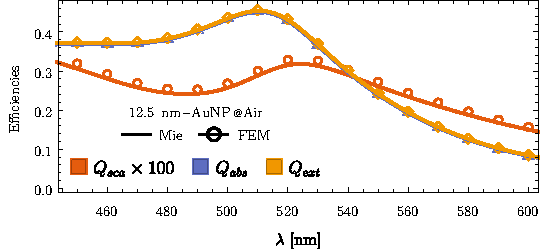
\includegraphics[width = .8\textwidth ]{1-Theory-Figs/Mie-FEM_Air.pdf}\\
%\includegraphics[width = .4\textwidth ]{1-Theory-Figs/Isolated-COMSOL.pdf}%
%\includegraphics[width = .4\textwidth ]{1-Theory-Figs/Isolated-COMSOL.pdf}%
%\caption[Convergence tests: The Meshing]{Resonance wavlength ($\lambda_\text{res}$) of the scattering (orange) and extinction (black) cross sections as functions of the NPs radii when embedded  \ref{sfig:red:1} into air and \ref{sfig:red:2} into water, and as function of the refractive index of the matrix for NP of radius set to  \ref{sfig:red:3} 12.5 nm and \ref{sfig:red:4} 50 nm.}
%\end{figure}




\begin{figure}[h!]\centering
	\def\svgwidth{.8\textwidth} \small
\includeinkscape{1-Theory-Figs/SistemaBox}
\vspace*{0em}
\caption[Spherical symmetric COMSOL Setup]{A 3D view (left) and the cross section (right) of a spherical symmetric COMSOL setup to calculate the optical response of a single spherical NP embedded into a matrix. The NP (yellow) is located at the center of the matrix (gray), which is covered by a PML layer (blue). The upper layer of the PML is hidden to allow a better view of the setup.}
\label{fig:setup:sphere}
\end{figure}

\begin{figure}[h!]
\def\svgwidth{\textwidth} \small
\hspace*{-1.25em}
\begin{subfigure}{.1\textwidth}\caption{ }\label{fig:Eff:sphere:First:a}\end{subfigure}
\vspace*{12.5em} % Crece la distancia entre as etiquetas
\\
\vspace*{-16.5em} % Crece la distancia entre las etiquetas y el pie de figura
\hspace*{-.75em}%
\begin{subfigure}{.1\textwidth}\caption{ }\label{fig:Eff:sphere:First:b}\end{subfigure}\\
\includeinkscape{1-Theory-Figs/4-Conv}
\vspace*{-1.5em} %Crece la ditancia entre la imagen y el pie de figura
\caption[Scattering, Absorption and Extinction Efficiencies of a 5 nm AuNP$@$Air: Analytical and FEM solutions with no optimizatio]{\textbf{a)} Scattering $Q_\text{sca}$, absorption $Q_\text{abs}$ and extinction $Q_\text{ext}$ efficiencies of a 5 nm AuNP embedded into air calculated by means of the Mie Theory (continuous) and the FEM (disks), and \textbf{b)} their absolute error, as function of the wavelength $\lambda$ of the incident planewave. The chosen parameters for the FEM calculations were based on the COMSOL Excercises \textbf{CITAR}.}
\label{fig:Eff:sphere:First}
\end{figure}


%

\chapter{Results and Discussion}
%	% !TeX root = ../tesis.tex

To compare the optical response of a NP in the presence of a substrate with that of a NP in a totally homogeneous environment, let us first analyze the spectral response given by the Mie Theory when the matrix and the size of the NP varies. In Fig. \ref{fig:Mie:redshift} it is shown the wavelength of resonance $\lambda_\text{res}$, that is, the wavelength at which the scattering (orange) and extinction (black) efficiencies are maximized,  as a  function of the radius $a$ of a AuNP embedded in a matrix of air [Fig. \ref{sfig:red:1}] and of glass [Fig. \ref{sfig:red:2}], with a refractive index of $n_\text{m} = 1$ and $n_\text{m} = 1.5$, respectively, and as a function of the refractive index of the matrix $n_\text{m}$ for a AuNP with a radius of {$a = 12.5$ nm} [Fig. \ref{sfig:red:3}] and with a radius of $a = 50$ nm [Fig. \ref{sfig:red:4}]. For the optical response of the AuNP it was employed the experimental data as reported (filled circles) by \citeauthor{johnson_optical_1972} \cite{johnson_optical_1972}  and by considering a size correction ---see Appendix \ref{app:SizeCorrection}--- to it (empty circles).

\begin{figure}[h!] \centering
    \def\svgwidth{.9\textwidth}
    \includeinkscape[pretex = \small]{Redshift/redshift}
    \vspace*{-18.6em} \\
    \hspace*{-5.9em}%
        \begin{subfigure}{.20\textwidth}\caption{ }\label{sfig:red:1}\end{subfigure}%
        \begin{subfigure}{.235\textwidth}\caption{ }\label{sfig:red:2}\end{subfigure}%
        \begin{subfigure}{.20\textwidth}\caption{ }\label{sfig:red:3}\end{subfigure}%
        \begin{subfigure}{.24\textwidth}\caption{ }\label{sfig:red:4}\end{subfigure}
    \vspace*{16.5em}\\
    \caption[Spectral redshift of the scattering and extinction  efficiencies of a spherical AuNP as a function of its size and the embedding media]{Resonance wavelength $\lambda_\text{res}$ of the scattering (orange) and extinction (black) efficiencies of a AuNP as a function of the NP's radius when embedded \textbf{a)} in air ($n_\text{m} = 1)$ and \textbf{b)} in glass ($n_\text{m} = 1.5$), and as a function of the refractive index of the matrix  $n_\text{m}$ for a AuNP of radius \textbf{c)} 12.5 nm and \textbf{d)} 50 nm, using the dielectric function for gold as reported by \citeauthor{johnson_optical_1972} (filled circle) and considering a size correction to it (empty circles).}
    \label{fig:Mie:redshift}
\end{figure}

\textcolor{red}{
From the results shown in Fig. \ref{fig:Mie:redshift} it can be seen that, in general, the wavelength of resonance  $\lambda_\text{res}$ for the extinction is smaller than for the scattering  and that the distance between them decreases as either the size of the AuNP or the refractive index of the matrix increases, meaning that the contribution of the scattering to the extinction of light becomes larger alongside these parameters, as discussed in Section \ref{ss:AuMie}. An increase in $a$ or in $n_\text{m}$ diminishes the difference between the results with and without a size correction, as shown in Figs. \ref{sfig:red:1}, \ref{sfig:red:2} and \ref{sfig:red:4},  however if these results are contrasted  it can be noted on the one hand that the resonance wavelength only redshifts as $a$ grows when no size correction is considered (filled cirlces) but that a size corrected dielectric function (empty circles) give rise to a blueshift of $\lambda_\text{res}$ for values of radius $\lessapprox 15/n_\text{m}$ as seen if Figs. \ref{sfig:red:1} and \ref{sfig:red:2}. On the other hand, an increase in $n_\text{m}$ for a fixed radius presents only redshifts either with or without a size corrected dielectric function [see Fig. \ref{sfig:red:3}].
}

The spectral behavior of the scattering and extinction of light due to a spherical NP summarized in Fig. \ref{fig:Mie:redshift} was calculated by assuming a homogeneous medium (the matrix) embedding the NP and thus allowing the direction of the illuminating plane wave to be arbitrary, yet yielding the same results. In the following sections, the homogeneity of the surroundings of the NP is substituted by two semiinfinite media and thus modifying the optical response of the system depending on how it is illuminated.

	\section{Incrustation Degree of a Spherical Particle}
%	% !TeX root = ../tesis.tex


\chapter{Results}

\section{What I got}
\label{section:results}
				
\Blindtext

    \section{Future Work: Application on Metasurfaces}

\chapter{Conclusions}


\appendix

\chapter{Mie Theory (Conventions and Code)}
  \label{app:MieCode}
  % !TeX root = ../tesis.tex

The Vector Spherical Harmonics (VSH) where defined in Sec. \ref{ssection:VSH} in terms of their generating function $\psi(r,\theta,\varphi)$ which must satisfy the scalar Helmholtz equation [Eq.  \eqref{eq:HelmoltzScalar}]. By employing the separation of variables method,  it was determined that $\psi$ is the product of either $\sin(m\varphi)$ or $\cos(m\varphi)$, of the associated Legendre functions $P_\ell^m(\cos\theta)$ and the spherical Bessel/Hankel functions $z_\ell(kr)$, all of which are solutions to Eqs. \eqref{eq:Phi}-\eqref{eq:Reqkr}. In this section, it is discussed the chosen definitions for $P_\ell^m$, $z_\ell$ and related functions, as well as how to calculate them. It is also detailed how to code the Mie Theory results employing the Wolfram Language.

\section*{Radial Dependency:\\ Spherical Bessel/Hankel Functions}

Te radial dependency of the VSH is given by the solutions to Eq. \eqref{eq:Reqkr} which are the spherical Bessel function of first and second kind $j_\ell(kr)$ and $y_\ell(kr)$, respectively, related by the regular Bessel function of fractional order $J_{\ell+1/2}(kr)$ and  $Y_{\ell+1/2}(kr)$ by
%
\begin{align}
j_\ell(kr) = \sqrt{\frac{\pi}{2(kr)}}J_{\ell+1/2}(kr),\qqtext{ and} 
y_\ell(kr) = \sqrt{\frac{\pi}{2(kr)}}JY{\ell+1/2}(kr),
\end{align}
%

\section*{Angular Dependency on $\theta$ and $\varphi$:\\ Sine, Cosine, Associated Legendre Functions and the Angular Functions $\pi_\ell$ and $\tau_\ell$}

Within this text, it was chosen the azimuthal solution to the scalar Helmholtz equation to be sines and cosines, so $m$ can only take non negative integer values. This functions obey the orthogonality relations
%
\begin{align}
\int_0^{2\pi} \sin(m\varphi)\sin(m'\varphi) \dd{\varphi} &=
\int_0^{2\pi} \cos(m\varphi)\cos(m'\varphi) \dd{\varphi} =\delta_{m,m'}( 1+ \delta_{0,m}) \pi,
\label{eq:SinCos}
\\
\int_0^{2\pi} \cos(m\varphi)\sin(m'\varphi) \dd{\varphi} &=0,
\end{align}
%
with $\delta_{m,m'}$ the Kroneker delta.

The solution to the polar angle equation are the associated Legendre functions and in this work they are defined as by \citeauthor{arfken_mathematical_2001} \cite{arfken_mathematical_2001}, that is,
%
\begin{equation}
P_\ell^m(\mu) = (1-\mu^2)^{m/2}\dv[m]{P_\ell(\mu)}{\mu},
\qqtext{ with}
P_\ell(\mu) = \frac{1}{2^\ell \ell!}\qty(\dv{\mu})^\ell(\mu^2-1)^\ell,
\label{eq:Plm}
\end{equation}
%
where $\mu = \cos\theta$ and $P_\ell(\mu)$ are the Legendre polynomials with $\ell$ also a non negative integer. With such definition, the  associated Legendre functions follows the orthogonality relation
%
\begin{align}
\int_{-1}^1 P_\ell^m(\mu)P_{\ell'}^m(\mu)\dd{\mu} = \frac{2\delta_{\ell,\ell'}}{2\ell+1}\frac{(\ell+m)!}{(\ell-m)!},
\label{eq:PlmOrtho}
\end{align}
%
To prove the orthogonality of $\pi_\ell(\mu)\pm\tau_\ell(\mu)$, with $\pi_\ell$  and $\tau_\ell$ the angular functions defined in Eq. \eqref{eq:PiTau}, let us apply the Legendre equation [Eq. \eqref{eq:Theta}] to $P_\ell^m$ and multiply it by $P_{\ell'}^m$; repeating this procedure inverting $\ell$ and $\ell'$ and adding both equations it is obtained that
%
\begin{align}
\dv{\theta}&\qty(\sin\theta P_{\ell'}^m(\mu)\dv{P_\ell^m(\mu)}{\theta}) +
\dv{\theta}\qty(\sin\theta P_{\ell}^m(\mu)\dv{P_{\ell'}^m(\mu)}{\theta}) +  
\label{eq:PlPl'}
\\
&\qty[\ell(\ell+1)+\ell'(\ell'+1)]P_{\ell'}^m(\mu)P_{\ell}^m(\mu) \sin\theta
=
 2\qty(\frac{mP_\ell^m(\mu)}{\sin\theta}\frac{mP_{\ell'}^m(\mu)}{\sin\theta}+ \dv{P_\ell^m(\mu)}{\theta}\dv{P_{\ell'}^m(\mu)}{\theta})\sin\theta,\notag
\end{align}
%
where  it was added $2\dv*{P_\ell^m}{\theta}\dv*{P_{\ell'}^m}{\theta}$ on both sides to complete the derivatives. Integrating Eq. \eqref{eq:PlPl'} in th interval $\theta \in (0,\pi)$, or $\mu \in(-1,1)$, and employing Eqs. \eqref{eq:Plm} and \eqref{eq:PlmOrtho}, one obtains that
%
\begin{align}
\int_{-1}^1 \qty(\frac{mP_\ell^m(\mu)}{\sin\theta}\frac{mP_{\ell'}^m(\mu)}{\sin\theta}+ \dv{P_\ell^m(\mu)}{\theta}\dv{P_{\ell'}^m(\mu)}{\theta})\dd{\mu} = 
\delta_{\ell,\ell'}\frac{2\ell(\ell+1)}{2\ell+1}\frac{(\ell+m)!}{(\ell-m)!}.
\label{eq:PimlTauml}
\end{align}
%
Additionally 
%
\begin{align}
\int_{-1}^1\frac{mP_\ell^m(\mu)}{\sin\theta}\dv{P_{\ell'}^m(\mu)}{\theta}\dd{\mu}
 = \int_0^{\pi} mP_\ell^m(\mu)\dv{P_{\ell'}^m(\mu)}{\theta}\dd{\theta} = 
 -\int_{-1}^1\frac{mP_{\ell'}^m(\mu)}{\sin\theta}\dv{P_{\ell}^m(\mu)}{\theta}\dd{\mu}.
 \label{eq:taupiCross}
\end{align}
%
where Eq. \eqref{eq:Plm} was employed along integration by parts. Thus, combining Eqs. \eqref{eq:PimlTauml} and \eqref{eq:taupiCross}, it leads to
%
\begin{align}
\int_{-1}^{1}\qty(\frac{mP_\ell^m(\mu)}{\sin\theta}\pm\dv{P_\ell^m(\mu)}{\theta})\qty(\frac{mP_{\ell'}^m(\mu)}{\sin\theta}\pm\dv{P_{\ell'}^m(\mu)}{\theta})\dd{\mu}  
 =  \delta_{\ell,\ell'}\frac{2\ell(\ell+1)}{2\ell+1}\frac{(\ell+m)!}{(\ell-m)!}.
 \label{eq:(pipmtau)}
\end{align}
%
The Eq. \eqref{eq:(pipmtau)}  is the orthogonality of $\pi_\ell(\mu)\pm\tau_\ell(\mu)$ when $m = 1$, which also simplifies the right hand side to $\delta_{\ell,\ell'} 2\ell^2(l+1)^2/(2\ell+1)$.

The angular functions $\pi_\ell(\tau)$ and $\tau_\ell(\mu)$ can be calculated recursively by taking advantage of the  recurrence relations of the Legendre polynomials \cite{arfken_mathematical_2001}
%
\begin{align}
(2\ell-1)\mu P_{\ell-1}(\mu) =& (\ell-1) P_{\ell}(\mu) + \ell P_{\ell-2}(\mu),\\
(1-\mu)^2\dv{P_\ell(\mu)}{\mu} =& \ell P_{\ell-1}(\mu) - \ell\mu P_\ell(\mu),
\end{align}
%
and Eq. \eqref{eq:Plm} with $m=1$, which also implies that  $\pi_1(\mu) = 1$. By defining $\pi_0(\mu)=0$, then
%
\begin{align}
\pi_\ell(\mu) =& \frac{2\ell-1}{\ell-1}\mu \pi_{\ell-1}(\mu) - \frac{\ell}{\ell-1}\pi_{\ell-2},\\
\tau_ \ell (\mu) =& \ell\mu\pi_\ell(\mu) - (\ell+1)\pi_{\ell-2}(\mu).
\end{align}
%

\begin{mmaCell}[
	pattern = {n, th,n_,th_},
	local = {pi}
	]{Code}
  (*Angular functions pi and tau - n-> order - th -> polar angle theta*)
  MiePi[n_, th_] := Module[{pi}, 
     pi[0] = 0; pi[1]= 1;  
     pi[\mmaPat{i_}]:= pi[i] = ((2i-1)/(i-1))*Cos[th]*pi[i-1]-(i/(i-1))*pi[i-2]; 
    pi[n]]
     
  MieTau[n_, th_] := Module[{pi}, 
     pi[0] = 0; pi[1]= 1;  
     pi[\mmaPat{i_}]:= pi[i] = ((2i-1)/(i-1))*Cos[th]*pi[i-1]-(i/(i-1))*pi[i-2]; 
    n*Cos[th]*pi[n]-(n+1)*pi[n - 1]]

		SetAttributes[MiePi, Listable]
		SetAttributes[MieTau, Listable]
\end{mmaCell}

Another notable result from Eq. \eqref{eq:Plm} is that the angular functions $\pi_\ell(\mu)$ and $\tau_\ell(\mu)$ when evaluated at $\theta =0$ ($\mu = 1$)  follows 
%
\begin{align}
\pi_\ell(\mu=1) & =  \dv{P_\ell(\mu)}{\mu}\eval_{\mu=1},\\
\tau_\ell (\mu = 1) & = \qty[\dv{P_\ell^1(\mu)}{\mu} + (1-\mu^2)^{1/2}\dv[2]{P_\ell(\mu)}{\mu}]\eval_{\mu=1} = \dv{P_\ell(\mu)}{\mu}\eval_{\mu=1},
\end{align}
%
which can be obtained from the Legendre equation  by setting $m = 1$ and $\mu = 1$ in Eq. \eqref{eq:ThetaMu}, leading to
%
\begin{align}
\pi_\ell(\mu=1) = \tau_\ell(\mu=1) = \frac{\ell(\ell+1)}{2} P_\ell(\mu = 1) = \frac{\ell(\ell+1)}{2},
\end{align}
%
where the last equality arises from the chosen definition of the Legendre polynomial [Eq. \eqref{eq:Plm}].

	\section*{Radial functions and Mie Coefficients}










\section*{Vector Spherical Harmonics Orthogonality Relations}

The VSH follow orthogonality relations inherited from the orthogonality of sine, cosine and the associated Legendre functions. Let us define the inner product as the integral in the solid angle between two vector functions as 
%
\begin{align}
\ev{\vb{A},\vb{A}'}_\Omega = \int_0^{2\pi}\int_0^{\pi} \vb{A}\cdot\vb{A}'\sin\theta\dd{\theta}\dd{\varphi}.
\label{eq:inner}
\end{align}
%
Under this inner product, all even VSH are orthogonal to the odd VSH due to the orthogonality of $\sin(m\varphi)$ and $\cos(m'\varphi)$, as well as all VSH  with $m\neq m'$ [Eq. \eqref{eq:SinCos}]. The remaining orthogonality relations  can be obtained by considering Eq. \eqref{eq:PimlTauml}, leading to 
%
\begin{align}
\ev{\vb{L}_{em'\ell},\vb{L}_{em'\ell'}}_\Omega &= \ev{\vb{L}_{om\ell},\vb{L}_{om\ell'}}_\Omega \notag\\
 &=  \delta_{m,m'}\delta_{\ell,\ell'} (1+\delta_{m,0}) 
 \frac{2\pi}{2\ell+1}\frac{(\ell+m)!}{(\ell-m)!}
 \qty[\qty(k\dv{z_\ell(kr)}{(kr)})^2 + \ell(\ell+1)\qty(k\frac{z_\ell(kr)}{kr})^2],\\
\ev{\vb{M}_{em\ell},\vb{M}_{em\ell'}}_\Omega &= \ev{\vb{M}_{om\ell},\vb{M}_{om\ell'}}_\Omega \notag\\
&= \delta_{m,m'}\delta_{\ell,\ell'} (1+\delta_{m,0}) 
\pi \frac{2  \ell(\ell+1)}{2\ell+1}\frac{(\ell+m)!}{(\ell-m)!}
z_{\ell}^2(kr),\\
%
\ev{\vb{N}_{em\ell},\vb{N}_{em\ell'}}_\Omega &= \ev{\vb{N}_{om\ell},\vb{N}_{om\ell'}}_\Omega  \notag\\
&= \delta_{m,m'}\delta_{\ell,\ell'} (1+\delta_{m,0}) 
\pi \frac{2  \ell(\ell+1)}{2\ell+1}\frac{(\ell+m)!}{(\ell-m)!}
\qty[\qty(\frac{ z_{\ell}}{kr})^2 + \qty(\frac{1}{kr}\dv{[kr z_\ell(kr)]}{(kr)})^2]. \\
%%
\ev{\vb{L}_{em\ell},\vb{N}_{em\ell'}}_\Omega &= \ev{\vb{L}_{om\ell},\vb{N}_{om\ell'}}_\Omega \notag\\
&= \delta_{m,m'}\delta_{\ell,\ell'} (1+\delta_{m,0}) 
\pi \frac{2  \ell(\ell+1)}{2\ell+1}\frac{(\ell+m)!}{(\ell-m)!}
\qty[\frac{ z_{\ell}}{kr}\dv{z_\ell(kr)}{(kr)} + \qty(\frac{1}{kr}\dv{[kr z_\ell(kr)]}{(kr)})^2]
\end{align}
%



%
\begin{align}
\ev{\vb{L}_{em\ell},\vb{L}_{em\ell'}}_\Omega = \ev{\vb{L}_{om\ell},\vb{L}_{om\ell'}}_\Omega &= 
		\delta_{\ell,\ell'}\frac{(1+\delta_{m,0})2\pi}{2\ell+1}\frac{(\ell+m)!}{(\ell-m)!}k^2\qty[ \ell z_{\ell-1}^2(kr) + (\ell+1)z_{\ell+1}^2(kr) ],\\
%
\ev{\vb{N}_{em\ell},\vb{N}_{em\ell'}}_\Omega = \ev{\vb{N}_{om\ell},\vb{N}_{om\ell'}}_\Omega &= \delta_{\ell,\ell'}\frac{(1+\delta_{m,0})2\pi}{(2\ell+1)^2}\frac{(\ell+m)!}{(\ell-m)!}\ell(\ell+1)\qty[ (\ell+1) z_{\ell-1}^2(kr) + \ell z_{\ell+1}^2(kr) ]. \\
%%
\ev{\vb{L}_{em\ell},\vb{N}_{em\ell'}}_\Omega = \ev{\vb{L}_{om\ell},\vb{N}_{om\ell'}}_\Omega &= \delta_{\ell,\ell'}\frac{(1+\delta_{m,0})2\pi}{(2\ell+1)^2}\frac{(\ell+m)!}{(\ell-m)!}\ell(\ell+1)k\qty[ z_{\ell-1}^2(kr) - z_{\ell+1}^2(kr) ]. 
\end{align}
%

























\chapter{Size Corrected Dielectric Function}
  \label{app:SizeCorrection}
  % !TeX root = ../tesis.tex

In this work, the optical properties of spherical gold (Au) nanoparticles (NPs) with radius $a = 12.5$ nm were studied. Even though the optical response of a non magnetic material is codified into the dielectric function $\varepsilon(\omega)$, the dielectric function for materials at the nanoscale differs from those in bulk due to surface effects. To perform a size correction to the dielectric function, let us decompose it into two additive contributions arising from intra- and interband electronic transitions \cite{noguez_surface_2007}. If no spacial dispersion is considered, the intraband contribution of the dielectric function can be described by means of the Drude-Sommerfeld model 
%
\begin{align}
\frac{\varepsilon_\text{\scriptsize Drude}(\omega)}{\varepsilon_0} = 1 - \frac{\omega_p^2}{\omega(\omega + i \gamma)},
\label{eq:Drude}
\end{align}
% 
where $\varepsilon_0$ is the vacuum permittivity, and $\omega_p$ is the plasma frequency and $\gamma$ the damping constant. In general, the damping constant is inversely proportional to the average time between collision events of the electrons inside the material and its value depends on the material itself and on its the geometry and dimensions. For example, the damping constant for a material in bulk $\gamma^\text{Bulk}$ equals $v_\text{F}/L$  with $v_\text{F}$ the Fermi velocity and $L$ the  mean free path of the electrons. On the other hand, the damping constant $\gamma^\text{NP}_a$ for a spherical NP of radius $a$ deviates from $\gamma^\text{Bulk}$ if the mean free path is greater than the size of the NP ($ L > 2a $), in which case an effective  mean free path replaces $L$, leading to the following expression for the damping constant:
%
\begin{align}
\gamma^\text{\scriptsize  NP}_a =  \gamma^\text{\scriptsize Bulk} + A\frac{v_\text{F}}{a},
\qqtext{ with }
\gamma^\text{\scriptsize  Bulk} = \frac{v_\text{F}}{L},
\label{eq:SC}
\end{align}
%
where $A$ is a theory dependent parameter whose exact value changes according to the approach employed to calculate the effective mean free path; for this work it is considered that $A = 1$. 

In practice, the experimental data for the dielectric function of a material $\varepsilon_\text{\scriptsize Exp}(\omega)$ corresponds to a material in bulk, so a size  correction is performed on $\varepsilon_\text{\scriptsize Exp}(\omega)$ if the optical properties of NPs are studied. The size correction is done by subtracting the intraband  contribution that best fits the experimental bulk data and adding an intraband contribution considering Eq. \eqref{eq:SC}, that is, the size corrected dielectric function  $\varepsilon_\text{\scriptsize Size}(\omega)$ is given by
%
\begin{align}
\frac{\varepsilon_\text{\scriptsize Size}(\omega)}{\varepsilon_0} = 
	\frac{\varepsilon_\text{\scriptsize Exp}(\omega)}{\varepsilon_0} +
 \qty(- 
	 \frac{\varepsilon_\text{\scriptsize Drude}(\omega)}{\varepsilon_0}
	 									\eval_{\gamma = \gamma^\text{\scriptsize  Bulk}}
	 +
	 \frac{\varepsilon_\text{\scriptsize Drude}(\omega)}{\varepsilon_0}
 										\eval_{\gamma = \gamma^\text{\scriptsize  NP}_a} 	 							),
 \label{eq:EpsSC}
\end{align}
%
The size correction in Eq. \eqref{eq:EpsSC} considers the size effects on the intraband contribution of the dielectric function while the size corrections due to the interband contributions are neglected since it has been reported that they are relevant for NPs with radii smaller than $2$ nm \cite{mendoza_herrera_determination_2014}. 

To employ the size corrected dielectric function [Eq. \eqref{eq:EpsSC}], the parameters  $\omega_p$ and $\gamma^\text{\scriptsize Bulk}$ that best fit  $\varepsilon_\text{\scriptsize Exp}(\omega)$ are needed. Let us develop two linear relations involving $\omega_p$ and $\gamma^\text{\scriptsize Bulk}$ and the real and imaginary parts of $\varepsilon_\text{\scriptsize Drude}(\omega)$ following the method from \citeauthor{mendoza_herrera_determination_2014}. The real and imaginary parts of $\varepsilon_\text{\scriptsize Drude}(\omega)$ are 
%
\begin{align}
\Re\qty[\frac{\varepsilon_\text{\scriptsize Drude}(\omega)}{\varepsilon_0}] = 1 - \frac{\omega_p^2 \omega^2}{\omega^4 + (\omega\gamma)^2},
\qqtext{ and}
\Im\qty[\frac{\varepsilon_\text{\scriptsize Drude}(\omega)}{\varepsilon_0}]  = \frac{\omega_p^2  (\omega\gamma)}{\omega^4 + (\omega\gamma)^2}.
\end{align}
%
according to Eq. \eqref{eq:Drude}. By multiplying the imaginary part of $\varepsilon_\text{\scriptsize Drude}(\omega)$ by $\omega$ and compairing it with its real part, one obtains that
%
\begin{align}
\omega \Im\qty[\frac{\varepsilon_\text{\scriptsize Drude}(\omega)}{\varepsilon_0}] =
 \gamma \qty(1 - \Re\qty[\frac{\varepsilon_\text{\scriptsize Drude}(\omega)}{\varepsilon_0}]),
\label{eq:gammaFit}
\end{align}
%
and in a similar manner it can be verified that
\begin{align}
\omega^2\left\{ \Im\qty[\frac{\varepsilon_\text{\scriptsize Drude}(\omega)}{\varepsilon_0}]^2
			+ \qty(1-\Re\qty[\frac{\varepsilon_\text{\scriptsize Drude}(\omega)}{\varepsilon_0}])^2 \right\}
 = \omega_p^2 \qty(1 - \Re\qty[\frac{\varepsilon_\text{\scriptsize Drude}(\omega)}{\varepsilon_0}]).
 \label{eq:wpFit}
\end{align}
%%
	\begin{figure}[b!]
	\def\svgwidth{.85\textwidth} \small\centering	
	\includeinkscape{5-Apendices-Figs/DrudeFit}
	\caption[Plasma frequency and damping constant determination for Au]{Plot of Eqs. \eqref{eq:gammaFit} (orange) and \eqref{eq:wpFit} (black) evaluated with the experimental dielectric function reported by \citeauthor{johnson_optical_1972} \cite{johnson_optical_1972}. The shaded region corresponds to the frequency window from $0.64$ eV to $1.76$ eV, which is best described by the Drude-Sommerfeld model and which was considered to perform the linear fits (dashed), determinating a plasma frequency of $\hbar\omega_p =(8.70\pm0.08)$ eV and a damping constant of $\hbar\gamma = (8.29 \pm 0.14)\times 10^{-2}$ eV for Au. }
	\label{fig:DrudeFit}
	\end{figure}	
%
%
By plotting the left hand side of Eqs. \eqref{eq:gammaFit} and \eqref{eq:wpFit} as a function of  $1-\Re[\varepsilon_\text{\scriptsize Drude}(\omega)/\varepsilon_0]$ and fitting two linear functions, the values for $\gamma$ and $\omega_p^2$ can be calculated according to the right hand side of Eqs. \eqref{eq:gammaFit} and \eqref{eq:wpFit}, respectively. As a final remark, the experimental dielectric function includes both an intra- and an interband contribution  while  Eqs. \eqref{eq:gammaFit} and \eqref{eq:wpFit} are only valid for the intraband contribution of the dielectric function, thus the linear fits should be done within an spectral window into which the interband contributions are negligible compared to the Drude-Sommerfeld model, which best describes the optical properties of a material  when $\omega\to 0$. The  chose of the spectral window for the experimental data fit of the dielectric function can modify the calculated values of $\gamma$ and $\omega_p$.
%


 In Fig. \ref{fig:DrudeFit}, the left hand side of Eqs. \eqref{eq:gammaFit}  and \eqref{eq:wpFit} are plotted in orange and black, respectively, as a function of $1-\Re[\varepsilon(\omega)/ \varepsilon_0]$, where $\varepsilon(\omega)$  corresponds to the experimental data of the dielectric function of Au (markers) reported by \citeauthor{johnson_optical_1972} \cite{johnson_optical_1972}; to ease the read of Fig. \ref{fig:DrudeFit}, continuous lines between the data were added as a guide to the eye and the photon energy $\hbar\omega$ of selected points of the experimental data are shown on the top margin. The shaded region in Fig. \ref{fig:DrudeFit} is the frequency window $0.64\text{ eV} < \hbar\omega < 1.76 \text{ eV}$, into which the experimental data for Au shows a linear behavior as stated by Eqs.\eqref{eq:gammaFit}  and \eqref{eq:wpFit}, that is, within this interval  the intraband contribution to the dielectric function is dominant, thus the linear fits (dashed lines) where made with the data in this region, determinating a plasma frequency of $\hbar\omega_p =(8.70\pm0.08)$ eV and a damping constant of $\hbar\gamma = (8.29 \pm 0.14)\times 10^{-2}$ eV for Au in bulk. Once the plasma frequency and the damping constant for Au have been obtained, the size corrected dielectric for spheres can be calculated. 

	\begin{figure}[b!]
	\def\svgwidth{.85\textwidth} \centering \small
	\includeinkscape{5-Apendices-Figs/JC}
	\caption[Au size corrected dielectric function]{ Real (blue) and imaginary (red) parts of the size corrected dielectric function of Au in bulk (continuous lines) and  of spherical Au NPs of radius $5$ nm (dotted lines), $12.5$ nm (dash dotted lines) and $80$ nm (dashed lines), as function of the photon energy $\hbar\omega$ (wavlength $\lambda$). The size corrected dielectric function was calculated from the experimental data of \citeauthor{johnson_optical_1972} \cite{johnson_optical_1972}. }
	\label{fig:EpsSize}
	\end{figure}


The real part (blue) and imaginary part (red) of the size corrected dielectric function for Au, based in the experimental data from \citeauthor{johnson_optical_1972},  is plotted in Fig. \ref{fig:EpsSize} as function of the photon energy $\hbar\omega$; on the top margin it is shown the convertion of the phton energy into wavelength $\lambda$. The size corrected dielectric function was calculated for several cases: Au in bulk (continuous lines) and  spherical Au NPs of radius $5$ nm (dotted lines), $12.5$ nm (dash dotted lines) and $80$ nm (dashed lines); all lines are guides to the eye. The data in  Fig. \ref{fig:EpsSize} shows that the need for a size corrected dielectric functions increases as the frequency decreases (wavelength decreases), specifically for the visible spectrum (shaded region) the size correction is appreciated for $\hbar \omega < 2.5$ eV ($\lambda>500$ nm). From Fig. \ref{fig:EpsSize} it can also be seen that the imaginary part of the size corrected dielectric function differs the most from the bulk dielectric function compared to its real part, whose deflection from the bulk optical response are barely visible near $\hbar\omega\approx 1$ eV.



%
%\begin{figure}
%\def\svgwidth{\textwidth} \centering \small
%\includeinkscape{5-Apendices-Figs/DrudeJC}
%\caption{   }
%\end{figure}







%%-------------------------------------------------------------------------------
%%                               References                                   |
%%-------------------------------------------------------------------------------
%
%\appendix
%% !TeX root = ../tesis.tex


\chapter{What I couldn't get into the main part}

\label{section:apendix1}
				
\Blindtext


\setlength\bibitemsep{.1\itemsep}
\printbibliography

\newpage
%: ----------------------- list of figures/tables ------------------------
\listoffigures              % Genera el ínidce de figuras, comentar línea si no se usa
%\listoftables               % Genera índice de tablas, comentar línea si no se usa
\printindex
%-------------------------------------------------------------------------------
%                              Appendix                                   |
%-------------------------------------------------------------------------------



\end{document}
